\documentclass[]{article}


%-----------------------------------------------------------------------------------------------------------------------------------------
%
%   GLOBALS
%
%-----------------------------------------------------------------------------------------------------------------------------------------
\newcommand{\DOCTITLE}{

}
\newcommand{\DOCAUTHOR}{

}
\newcommand{\DISCLAIMER}
{
    \topskip0pt
    \vspace*{\fill}
    {
    \centering
        \small{
            THIS DOCUMENT IS INTENDED FOR INTERNAL USE ONLY
        }
    }
    \\
    {
    \centering
        \small{
        UNAUTHORIZED DISTRIBUTION OF THIS DOCUMENT IS STRICTLY PROHIBITED 
        }
    }
    \vspace*{\fill}
}

\usepackage{lmodern}
\usepackage{amssymb,amsmath}
\usepackage{ifxetex,ifluatex}
\usepackage{fixltx2e} % provides \textsubscript
\ifnum 0\ifxetex 1\fi\ifluatex 1\fi=0 % if pdftex
  \usepackage[T1]{fontenc}
  \usepackage[utf8]{inputenc}
\else % if luatex or xelatex
  \ifxetex
    \usepackage{mathspec}
    \usepackage{xltxtra,xunicode}
  \else
    \usepackage{fontspec}
  \fi
  \defaultfontfeatures{Mapping=tex-text,Scale=MatchLowercase}
  \newcommand{\euro}{€}
\fi
% use upquote if available, for straight quotes in verbatim environments
\IfFileExists{upquote.sty}{\usepackage{upquote}}{}
% use microtype if available
\IfFileExists{microtype.sty}{%
\usepackage{microtype}
\UseMicrotypeSet[protrusion]{basicmath} % disable protrusion for tt fonts
}{}
\ifxetex
  \usepackage[setpagesize=false, % page size defined by xetex
              unicode=false, % unicode breaks when used with xetex
              xetex]{hyperref}
\else
  \usepackage[unicode=true]{hyperref}
\fi
\usepackage[usenames,dvipsnames]{color}
\hypersetup{breaklinks=true,
            bookmarks=true,
            pdfauthor={},
            pdftitle={},
            colorlinks=true,
            citecolor=blue,
            urlcolor=blue,
            linkcolor=magenta,
            pdfborder={0 0 0}}
\urlstyle{same}  % don't use monospace font for urls
\usepackage{color}
\usepackage{fancyvrb}
\newcommand{\VerbBar}{|}
\newcommand{\VERB}{\Verb[commandchars=\\\{\}]}
\DefineVerbatimEnvironment{Highlighting}{Verbatim}{commandchars=\\\{\}}
% Add ',fontsize=\small' for more characters per line
\newenvironment{Shaded}{}{}
\newcommand{\KeywordTok}[1]{\textcolor[rgb]{0.00,0.44,0.13}{\textbf{{#1}}}}
\newcommand{\DataTypeTok}[1]{\textcolor[rgb]{0.56,0.13,0.00}{{#1}}}
\newcommand{\DecValTok}[1]{\textcolor[rgb]{0.25,0.63,0.44}{{#1}}}
\newcommand{\BaseNTok}[1]{\textcolor[rgb]{0.25,0.63,0.44}{{#1}}}
\newcommand{\FloatTok}[1]{\textcolor[rgb]{0.25,0.63,0.44}{{#1}}}
\newcommand{\ConstantTok}[1]{\textcolor[rgb]{0.53,0.00,0.00}{{#1}}}
\newcommand{\CharTok}[1]{\textcolor[rgb]{0.25,0.44,0.63}{{#1}}}
\newcommand{\SpecialCharTok}[1]{\textcolor[rgb]{0.25,0.44,0.63}{{#1}}}
\newcommand{\StringTok}[1]{\textcolor[rgb]{0.25,0.44,0.63}{{#1}}}
\newcommand{\VerbatimStringTok}[1]{\textcolor[rgb]{0.25,0.44,0.63}{{#1}}}
\newcommand{\SpecialStringTok}[1]{\textcolor[rgb]{0.73,0.40,0.53}{{#1}}}
\newcommand{\ImportTok}[1]{{#1}}
\newcommand{\CommentTok}[1]{\textcolor[rgb]{0.38,0.63,0.69}{\textit{{#1}}}}
\newcommand{\DocumentationTok}[1]{\textcolor[rgb]{0.73,0.13,0.13}{\textit{{#1}}}}
\newcommand{\AnnotationTok}[1]{\textcolor[rgb]{0.38,0.63,0.69}{\textbf{\textit{{#1}}}}}
\newcommand{\CommentVarTok}[1]{\textcolor[rgb]{0.38,0.63,0.69}{\textbf{\textit{{#1}}}}}
\newcommand{\OtherTok}[1]{\textcolor[rgb]{0.00,0.44,0.13}{{#1}}}
\newcommand{\FunctionTok}[1]{\textcolor[rgb]{0.02,0.16,0.49}{{#1}}}
\newcommand{\VariableTok}[1]{\textcolor[rgb]{0.10,0.09,0.49}{{#1}}}
\newcommand{\ControlFlowTok}[1]{\textcolor[rgb]{0.00,0.44,0.13}{\textbf{{#1}}}}
\newcommand{\OperatorTok}[1]{\textcolor[rgb]{0.40,0.40,0.40}{{#1}}}
\newcommand{\BuiltInTok}[1]{{#1}}
\newcommand{\ExtensionTok}[1]{{#1}}
\newcommand{\PreprocessorTok}[1]{\textcolor[rgb]{0.74,0.48,0.00}{{#1}}}
\newcommand{\AttributeTok}[1]{\textcolor[rgb]{0.49,0.56,0.16}{{#1}}}
\newcommand{\RegionMarkerTok}[1]{{#1}}
\newcommand{\InformationTok}[1]{\textcolor[rgb]{0.38,0.63,0.69}{\textbf{\textit{{#1}}}}}
\newcommand{\WarningTok}[1]{\textcolor[rgb]{0.38,0.63,0.69}{\textbf{\textit{{#1}}}}}
\newcommand{\AlertTok}[1]{\textcolor[rgb]{1.00,0.00,0.00}{\textbf{{#1}}}}
\newcommand{\ErrorTok}[1]{\textcolor[rgb]{1.00,0.00,0.00}{\textbf{{#1}}}}
\newcommand{\NormalTok}[1]{{#1}}
\usepackage{longtable,booktabs}
\usepackage{graphicx,grffile}
\makeatletter
\def\maxwidth{\ifdim\Gin@nat@width>\linewidth\linewidth\else\Gin@nat@width\fi}
\def\maxheight{\ifdim\Gin@nat@height>\textheight\textheight\else\Gin@nat@height\fi}
\makeatother
% Scale images if necessary, so that they will not overflow the page
% margins by default, and it is still possible to overwrite the defaults
% using explicit options in \includegraphics[width, height, ...]{}
\setkeys{Gin}{width=\maxwidth,height=\maxheight,keepaspectratio}
\setlength{\parindent}{0pt}
\setlength{\parskip}{6pt plus 2pt minus 1pt}
\setlength{\emergencystretch}{3em}  % prevent overfull lines
\providecommand{\tightlist}{%
  \setlength{\itemsep}{0pt}\setlength{\parskip}{0pt}}
\setcounter{secnumdepth}{0}

\date{}

% Redefines (sub)paragraphs to behave more like sections
\ifx\paragraph\undefined\else
\let\oldparagraph\paragraph
\renewcommand{\paragraph}[1]{\oldparagraph{#1}\mbox{}}
\fi
\ifx\subparagraph\undefined\else
\let\oldsubparagraph\subparagraph
\renewcommand{\subparagraph}[1]{\oldsubparagraph{#1}\mbox{}}
\fi

%-----------------------------------------------------------------------------------------------------------------------------------------
%
%   PAGE SIZE AND MARGINS
%
%-----------------------------------------------------------------------------------------------------------------------------------------
\usepackage[a4paper,headheight=30pt]{geometry}
%\usepackage[letterpaper, portrait, margin=2in]{geometry}
\addtolength{\topmargin}{-.5in}
\addtolength{\textheight}{1.75in}

\usepackage{graphicx}

\usepackage{fancyhdr}
\pagestyle{fancy}


%-----------------------------------------------------------------------------------------------------------------------------------------
% Page break after sections
%-----------------------------------------------------------------------------------------------------------------------------------------
%\usepackage{titlesec}
%\newcommand{\sectionbreak}{\clearpage}

\lhead{
    %left header content
%    \topskip0pt
%    \vspace*{\fill}
    {
    \centering
        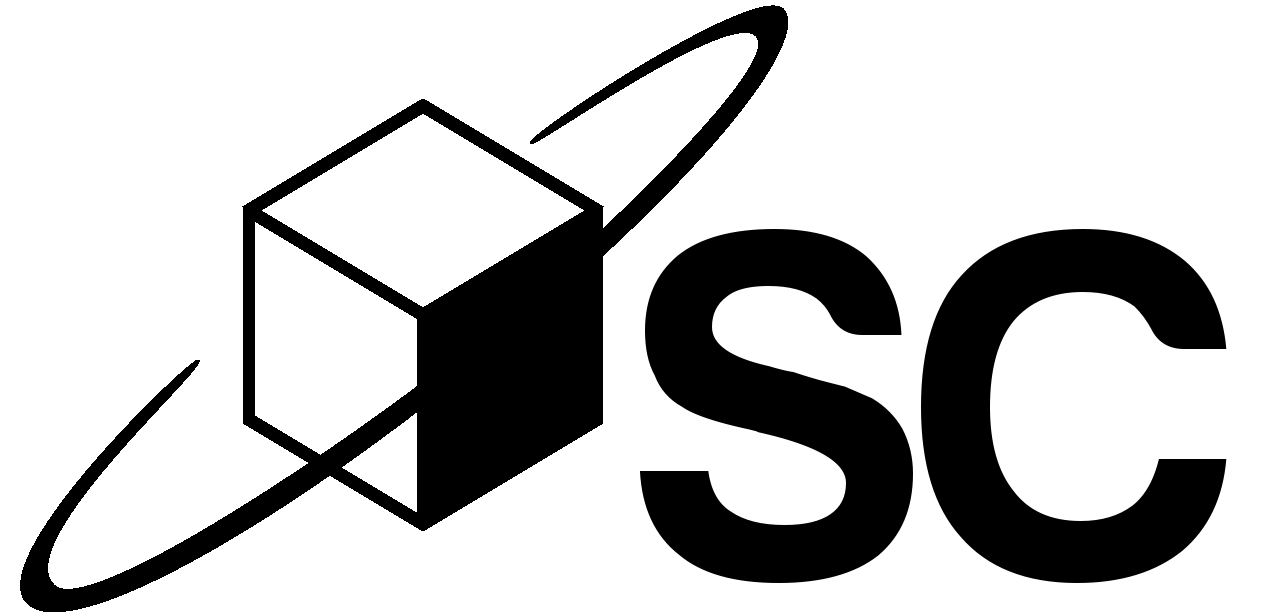
\includegraphics[height=2.66em]{template/sc.png}
    }
%    \vspace*{\fill}
}
\chead{
    \topskip0pt
    \vspace*{\fill}
    {
    \centering
        \small{
            THIS DOCUMENT IS INTENDED FOR INTERNAL USE ONLY
        }
    }
    \\
    {
    \centering
        \small{
        UNAUTHORIZED DISTRIBUTION OF THIS DOCUMENT IS STRICTLY PROHIBITED 
        }
    }
    \vspace*{\fill}
}
\rhead{
%    \topskip0pt
%    \vspace*{\fill}
    % right header content
    {
    \centering
        
\includegraphics[height=3.25em]{template/scrd.png}
    }
%    \vspace*{\fill}
}
\lfoot{
    % left footer content
    \topskip0pt
    \vspace*{\fill}
    SCRD
    Revision 0.1
    \vspace*{\fill}
}
\cfoot{
    % middle footer content
    \topskip0pt
    \vspace*{\fill}
    {
    \centering
    SCRD Internal Documents Template \\
    \today
    }
    \vspace*{\fill}
}
\rfoot{
    % right footer content
    \topskip0pt
    \vspace*{\fill}
    \thepage
    \vspace*{\fill}
}
% extend the header into the margins
\usepackage{calc}
\fancyheadoffset[L,R]{\marginparsep+\marginparwidth}

%--------------------------------------------------------------------------------------------------------------
%	My Packages
%--------------------------------------------------------------------------------------------------------------
\usepackage{capt-of}

%--------------------------------------------------------------------------------------------------------------
%
%	BEGIN DOCUMENT
%
%--------------------------------------------------------------------------------------------------------------
\begin{document}


%--------------------------------------------------------------------------------------------------------------
%
%	TITLE PAGE
%
%--------------------------------------------------------------------------------------------------------------
\begin{titlepage}

\newcommand{\HRule}{\rule{\linewidth}{0.5mm}} % Defines a new command for the horizontal lines, change thickness here

\center % Center everything on the page
 
%----------------------------------------------------------------------------------------
%	HEADING SECTIONS
%----------------------------------------------------------------------------------------

\includegraphics[width=200pt,height=200pt]{../images/rocketry_logo_large.png}\\[1cm] % Include a department/university logo - this will require the graphicx package
\textsc{\Large Space Concordia - Rocketry Division}\\[0.5cm] % Major heading such as course name
\textsc{\large Aurelius CR-2-4G - Structural Team}\\[0.5cm] % Minor heading such as course title

%----------------------------------------------------------------------------------------
%	LOGO SECTION
%----------------------------------------------------------------------------------------

\begin{figure}[ht]
    \centering
    \includegraphics[height=100pt]{../images/vertical_model_simplified.png}\\
\end{figure}

%----------------------------------------------------------------------------------------
%	TITLE SECTION
%----------------------------------------------------------------------------------------

\HRule \\[0.6cm]
{ \Huge \bfseries 
Performance Model Specification
}\\[0.4cm] 

\HRule \\[1cm]
 
%----------------------------------------------------------------------------------------
%	AUTHOR SECTION
%----------------------------------------------------------------------------------------

\begin{minipage}{0.4\textwidth}
\begin{flushleft} \large
	\begin{tabular} {r l} 
        \emph{Author(s):} & Shawn Bulger	\\
	\end{tabular}
\end{flushleft}
\end{minipage}
~
\begin{minipage}{0.4\textwidth}
\begin{flushright} \large
	\begin{tabular} {r l} 
		\emph{Coordinator:} & Dr. Ashok Kaushal 		\\
		\emph{Supervisor:}  & Dr. Mehdi Hojjati 		\\
		\emph{EIR:}         & Dominic Ng  		        \\
	\end{tabular}
\end{flushright}
\end{minipage}\\[2cm]

%----------------------------------------------------------------------------------------
%	DATE SECTION
%----------------------------------------------------------------------------------------

{\large \today}\\[2cm] % Date, change the \today to a set date if you want to be precise

\vfill % Fill the rest of the page with whitespace

\end{titlepage}

{
\hypersetup{linkcolor=black}
\setcounter{tocdepth}{3}
\tableofcontents
\clearpage
}
\listoftables
\listoffigures
\clearpage
\subsection{List of Abbreviations}\label{list-of-abbreviations}

\begin{longtable}[c]{@{}llll@{}}
\toprule
Abbreviation & Description & Function of & Units\tabularnewline
\midrule
\endhead
AOA, \(\alpha\) & Angle of Attack & & radians\tabularnewline
COP & Center of pressure & & N/A\tabularnewline
COG & Center of gravity & time & N/A\tabularnewline
Re & Reynolds Number & \( \rho,\mu,\vec{v},L \) &
dimensionless\tabularnewline
\(Re_{crit}\) & Critical Reynolds Number & \( \rho,\mu,\vec{v},L \) &
dimensionless\tabularnewline
\(I_{zz}\) & Pitch/Yaw Moment of Inertia & time & \(m^4\)\tabularnewline
D & Drag Force (combined) & & N\tabularnewline
W & Weight of the Rocket & & N\tabularnewline
R & Specific Gas Constant & & \(J kg^{-1} K^{-1}\)\tabularnewline
T & Thrust of the Rocket & & N\tabularnewline
\(t_f\) & Fin thickness & distance & m\tabularnewline
\(L_{cf}\) & Aerodynamic Chord Length of Fins & distance &
m\tabularnewline
c & Speed of sound & \( \sqrt{\gamma RT} \) &\tabularnewline
\(R_a\) & Surface Finish & \( distance \) & microns\tabularnewline
M & Mach Number & \( \vec{v}, c \) & dimensionless\tabularnewline
\(D_{pa}, C_{pa}\) & Parasitic Drag Force, Coefficient &
&\tabularnewline
\(D_{fb}, C_{fb}\) & Body Drag Force, Coefficient & &\tabularnewline
\(D_{fp}, C_{fp}\) & Fin Pressure Drag Force, Coefficient &
&\tabularnewline
\(D_{pr}, C_{pr}\) & Pressure Drag Force, Coefficient & &\tabularnewline
\(D_{in}, C_{in}\) & Interference Drag Force, Coefficient &
&\tabularnewline
\(D_{ba}, C_{ba}\) & Base Drag Force, Coefficient & &\tabularnewline
\(D_{sk}, C_{sk}\) & Skin Friction Drag Force, Coefficient &
&\tabularnewline
\(A_{wb}\) & Area of Wetted Body & &\tabularnewline
\(A_{wf}\) & Area of Wetted Fins & &\tabularnewline
\(A_{fr}\) & Frontal Reference Area & &\tabularnewline
OD,\(\phi_{bt}\) & Outer Diameter & & m\tabularnewline
L & Total Length of Rocket & & m\tabularnewline
h\_n & Height ofthe nose cone & & m\tabularnewline
\(S_{fc}\) & Thrust Specific Fuel Consumption & &
\(\dfrac{g}{s}\cdot \dfrac{1}{N} = \dfrac{s}{m}\)\tabularnewline
\(\dot{m}_{fc}\) & Mass Flow Rate due to Fuel Consumption & &
\(\dfrac{g}{s}\cdot \dfrac{1}{N} = \dfrac{s}{m}\)\tabularnewline
\(T_{avg}\) & Average Thrust & & N\tabularnewline
\(t_{burn}\) & Burn Time & & s\tabularnewline
\(m_{m_t}\) & Total Motor Mass & & g\tabularnewline
\(W_{m_t}\) & Total Motor Weight & & N\tabularnewline
\(F_N\) & Aerodynamic Normal Force & & N\tabularnewline
\(F_A\) & Aerodynamic Axial Force & & N\tabularnewline
\(F_L\) & Aerodynamic Lift Force & & N\tabularnewline
\(S_{lm}\) & Longitudinal Stability Margin & & Calibers\tabularnewline
\(f_B\) & Fineness Ratio & & dimensionless\tabularnewline
\(\mu\) & Dynamic Viscosity & & \(N s / m^2\)\tabularnewline
\(\nu\) & Kinematic Viscosity & \(\mu\), \(\rho\) &
\(m^2/s\)\tabularnewline
\bottomrule
\end{longtable}

\captionof{table}{List of Abbreviations}

\clearpage

\section{Performance Model
Specification}\label{performance-model-specification}

\subsection{Overview}\label{overview}

The goal of this project is to create a Performance Model in Matlab to
simulate the rocket flight characteristics.

Specifically the model should verify the maximum altitude and velocity.
Further developments are explored for future enhancement. A modular
development pattern will be followed order to support future expansion.
Unit testing of simulator logic will be undertaken where reasonable, and
further validation will be provided by testing the overall model against
3rd party flight data where available.

The model must take as input the current structural design parameters,
thrust information, and simulated ambient conditions of the launch
environment. Certain parameters will be dynamic; as the motor expends
fuel, the position of the center of gravity and center of pressure will
shift with decreasing mass. Additionally the moments of inertia will be
altered. These dynamic parameters must be considered to maximize the
accuracy of the model.

\subsection{Assumptions}\label{assumptions}

\begin{itemize}
\tightlist
\item
  subsonic flight
\item
  axis-symmetric rigid body rocket
\item
  single cylindrical body
\item
  Von Karman nose shape
\item
  three or four trapezoidal fins
\item
  passively controlled (no active thrust or stability control)
\item
  constant fuel expenditure rate
\item
  vertical/linear flight within 5 degrees {[}1{]}
\item
  the \emph{Ideal Gas Law} applies throughout the flight
\item
  humidity in the air is ignored
\item
  steady-state irrotational flow around the body {[}2{]}
\item
  fully aligned thrust {[}1{]}
\item
  smooth transition between nose cone and body tube (no shoulder)
\item
  rocket does not have a boattail
\item
  rocket has a single rectangular launch lug
\end{itemize}

\subsection{Requirements}\label{requirements}

The Performance Model must provide the maximum altitude and velocity of
the rocket in subsonic flight under a known thrust curve and known
dimensional parameters. Assumptions considered legitimate based on prior
research for similar rockets may be applied

\begin{itemize}
\tightlist
\item
  2a Static stability between 2 and 3 calibers
\item
  2b Dynamic stability above 0
\item
  2c Max velocity at launch rail 30.5 m/s
\item
  2d Vehicle max speed mach 0.9
\item
  2e Vehicle reaches 10,000 ft altitude (+1000 feet / - 0 feet)
\item
  2f Vehicle doesn't experience resonant pitching/yawing moment
\end{itemize}

{[}SCRD 2016 Specifications and Requirements{]}

\subsection{Validation}\label{validation}

\begin{itemize}
\tightlist
\item
  Sub-Models will be unit tested with 3rd party data to ensure
  functional validity where possible.
\item
  Once all Sub-Models are validated individually, the overall model will
  be validated using 3rd-party data.

  \begin{itemize}
  \tightlist
  \item
    Primary 3rd-party simulation data source will be OpenRocket
    simulations
  \item
    Where possible, actual 3rd-party rocket flight data will be used to
    validate the model
  \end{itemize}
\end{itemize}

\section{Input Parameters}\label{input-parameters}

Before beginning the modeling process, it is necessary to understand the
inputs of the system.

Many parameters can be considered unchanging during flight, and are from
this point referred to as \emph{Static Parameters}. Other inputs change
as a function of time or velocity, and must be carefully handled within
the system - these parameters are herein referred to as \emph{Dynamic
Parameters}.

The following table lists all input parameters to the system

\captionof{table}{Input Parameters}

\begin{longtable}[c]{@{}llll@{}}
\toprule
Parameter & Units & Status & Source\tabularnewline
\midrule
\endhead
area\_fin\_frontal & m\^{}2 & Static & CATIA\tabularnewline
area\_face\_fin & m\^{}2 & Static & CATIA\tabularnewline
width\_fins\_at\_tube & m & Static & CATIA\tabularnewline
fins\_count & N/A & Static & CATIA\tabularnewline
thickness\_fins\_at\_tube & m & Static & CATIA\tabularnewline
area\_surface\_nose & m\^{}2 & Static & CATIA\tabularnewline
height\_fins & m & Static & CATIA\tabularnewline
diameter\_outer & m & Static & CATIA\tabularnewline
surface\_roughness & m & Static & CATIA\tabularnewline
length\_total\_rocket & m & Static & CATIA\tabularnewline
pressure\_ambient\_ground & Pa & Static & Manual\tabularnewline
temperature\_ambient\_ground & C & Static & Manual\tabularnewline
distance\_tip\_to\_COG & m & Dynamic & CATIA\tabularnewline
distance\_tip\_to\_COP & m & Dynamic & Manual\tabularnewline
diameter\_outer\_launch\_guide & m & Static & CATIA\tabularnewline
diameter\_inner\_launch\_guide & m & Static & CATIA\tabularnewline
moment\_inertia\_rocket & m\^{}4 & Dynamic & CATIA\tabularnewline
\bottomrule
\end{longtable}

\begin{quote}
As agreed with Emily on 2015/10/02:
\end{quote}

\begin{quote}
\begin{itemize}
\tightlist
\item
  the parametric model must provide the moment of inertia, mass, area,
  and center of gravity of all static structural components (nose cone,
  body tube, fins, etc.)
\end{itemize}
\end{quote}

\begin{quote}
\begin{itemize}
\tightlist
\item
  the mass, center of mass (relative to the nose tip) of the motor
\end{itemize}
\end{quote}

These parameters are written in the parametric spreadsheet shared with
the design team. The CAD software populates values related to the
structural design, and others are entered manually. The performance
model reads them at the beginning of execution to simulate the latest
design iteration.

\subsection{Static Parameters}\label{static-parameters}

Much of the structural design of the rocket is unchanging during flight.

\subsection{Atmospheric Model}\label{atmospheric-model}

The \emph{International Standard Atmosphere} model is assumed to
describe the pressure, temperature, density and viscosity conditions of
the surrounding air during launch.

{[}3{]}

\subsubsection{Viscosity}\label{viscosity}

Previously, in-house simulations were conducted using the
\emph{velocity\_model} created by Alex Botros. Of interest to this
report, is the method by which the viscosity of the working fluid was
calculated. It will include a review of the previous methods use and it
will introduce \emph{Sutherland's law}. As well, both methods will be
compared and changes to the existing model will be proposed.

\subsubsection{Previous Work}\label{previous-work}

In the \emph{velocity\_model} the absolute viscosity was never actually
calculated. Instead, the kinematic viscosity was calculated (as shown
below) as part of the function to solve for the \emph{Reynolds Number}
of the vehicle.

\begin{equation}
\label{kinematic_viscosity_f_T}
\nu = (-1 E -14) T^3 + (1 E -10) T^2 + (3 E -8) T - (3 E -6)
\end{equation}

As can be clearly seen, the kinematic viscosity was estimated based on
the temperature T. It is assumed that the temperature is in Kelvin. When
the function shown here is plotted, it creates the following result.

\subsection{Dynamic Parameters}\label{dynamic-parameters}

Parameters listed as \emph{dynamic} in the table above are provided as
initial values which are then recalculated by the model throughout the
simulated flight.

\subsubsection{Thrust}\label{thrust}

Thrust is the mechanical force that drives the flight of the rocket. It
is a vector quantity of magnitude and direction. \emph{Thrust} is a
reaction force in the opposite direction of accelerating fluid (exhaust
gas) caused by the combustion of fuel.

\emph{Force} is a change in momentum with time, and is related by
Newton's Second Law

\begin{equation}
F = \dfrac{m \Delta \vec{v}}{\Delta t} = m\vec{a}
\end{equation}

\emph{Mass Flow Rate} is found by the product of fluid density,
velocity, and cross-sectional area.

\begin{equation} 
\dot{m} = \rho \vec{v} A
\end{equation}

\href{http://www.grc.nasa.gov/WWW/k-12/airplane/thrust1.html}{NASA -
Thrust}

\paragraph{Thrust Equation}\label{thrust-equation}

\begin{equation} 
T = \dot{m} \Delta \vec{v} 
\end{equation}

\href{http://www.grc.nasa.gov/WWW/k-12/airplane/thrsteq.html}{NASA -
Thrust Equation}

Thrust curves are provided by the manufacturer, and are rated at a
constant fuel expenditure rate known as the specific fuel consumption
(\(S_{fc}\))

Here is an example of the motor data provided by ThrustCurve.org:

\begin{longtable}[c]{@{}ll@{}}
\toprule
Parameter & Value\tabularnewline
\midrule
\endhead
Manufacturer & Cesaroni Technology\tabularnewline
Entered & May 20, 2009\tabularnewline
Last Updated & Jun 26, 2014\tabularnewline
Mfr. Designation & 6819M1540-P\tabularnewline
Common Name & M1540\tabularnewline
Motor Type & reload\tabularnewline
Delays & P\tabularnewline
Diameter & 75.0mm\tabularnewline
Length & 75.7cm\tabularnewline
Total Weight & 5906g\tabularnewline
Prop. Weight & 3624g\tabularnewline
Cert. Org. & Canadian Association of Rocketry\tabularnewline
Cert. Designation & 6819-M1540-IM-P\tabularnewline
Cert. Date &\tabularnewline
Average Thrust & 1537.0N\tabularnewline
Maximum Thrust & 2328.8N\tabularnewline
Total impulse & 6819.4Ns\tabularnewline
Burn Time & 4.4s\tabularnewline
Case Info & Pro75-5G\tabularnewline
Propellant Info & Imax\tabularnewline
Availability & regular\tabularnewline
\bottomrule
\end{longtable}

\captionof{table}{Sample Motor Data}

Source: http://www.thrustcurve.org/motorsearch.jsp?id=673

\subparagraph{Thrust Specific Fuel
Consumption}\label{thrust-specific-fuel-consumption}

\emph{Thrust Specific Fuel Consumption} is how much fuel is burned for a
given time.

\begin{equation}
S_{fg} = \dfrac{m}{t_{burn}}\cdot \dfrac{1}{T_{avg}}  
\end{equation}

\begin{equation}
\left[ \dfrac{g}{s}\cdot \dfrac{1}{N} = \dfrac{s}{m} \right]  
\end{equation}

Since at the time of writing the \(S_{fc}\) was not provided by the
manufacturer, the following calculations are used for a first
approximation.

Assumptions

\begin{itemize}
\tightlist
\item
  all propellant is spent during the motor burn time
\item
  final \(S_{fg}\) determined is constant during burn
\item
  the motor info provided is accurate
\end{itemize}

\begin{quote}
It should be noted that a variance in thrust of \(\pm 20 \%\) is
possible. This and other variance factors are taken into account in the
\emph{Statistical Analysis} section.
\end{quote}

From the table above, the dry propellant weight is given as 3624 grams.
The Average Thrust is given as 1537.0 Newtons, and the total burn time
is given as 4.4 seconds.

Thus, the \emph{Thrust Specific Fuel Consumption} can be determined as
follows:

\begin{equation}
S_{fg} = \dfrac{3.624 \, kg}{4.4 \, s} \cdot \dfrac{1}{1537.0 \, N} \approx 0.00053587 \dfrac{kg}{N \cdot s} = 5.3587 \times 10^{-4} \dfrac{kg}{N \cdot s} 
\end{equation}

This rate is considered constant.

\subsubsection{Weight}\label{weight}

As fuel is expended in generating thrust, the weight of the rocket is
reduced. We can use the \emph{Thrust Specific Fuel Consumption} to
determine the corresponding reduction in weight during burn.

First remove the Average Thrust term to isolate the mass flow rate:

\begin{equation}
\dot{m} = S_{fG} \cdot T_{avg} = 5.3587 \times 10^{-4} \dfrac{kg}{N \cdot s} \cdot 1537.0 \, N  = 0.8236 \, kg/s 
\end{equation}

This equation can be expressed in terms of Weight through Newton's
2\(^nd\) law: \(F = m\vec{a}\)

\begin{equation}
\dot{W}_m = \dot{m} \cdot \vec{g} = 0.8236 \, kg/s \cdot 9.81 \, m/s^2 \approx 8.0799 N/s 
\end{equation}

To develop a relation for the change in weight as a function of
\(S_{f_c}\)

\begin{equation} 
W_f(t) = (m_{f_i} kg - \Delta m(t)) \cdot \vec{g} 
\end{equation}

\begin{equation}
W_f(t) = (3.624 \, kg - \Delta m(t)) \cdot 9.81 \, m/s^2 
\end{equation}

\begin{equation}
W_f(t) = W_{f_i} - \Delta W_f(t)
\end{equation}

\begin{equation}
\Delta W_f (t) = \int \dot{W} dt = \dot{W}\cdot t
\end{equation}

\begin{equation}
\Delta W_f (t) = \dfrac{\Delta m(t) \cdot \vec{g}}{t}\cdot t = \Delta m (t) \cdot g 
\end{equation}

\begin{equation}
\Delta m_f(t) = S_{fg} \cdot t
\end{equation}

Finally, the motor weight as a function of time is

\begin{equation}
W_m (t) = W_{m_t} - \Delta W_f(t) = W_{m_t} - \dot{m}_{fc} \cdot t
\end{equation}

\paragraph{Matlab Implementation}\label{matlab-implementation}

\begin{figure}[htbp]
\centering
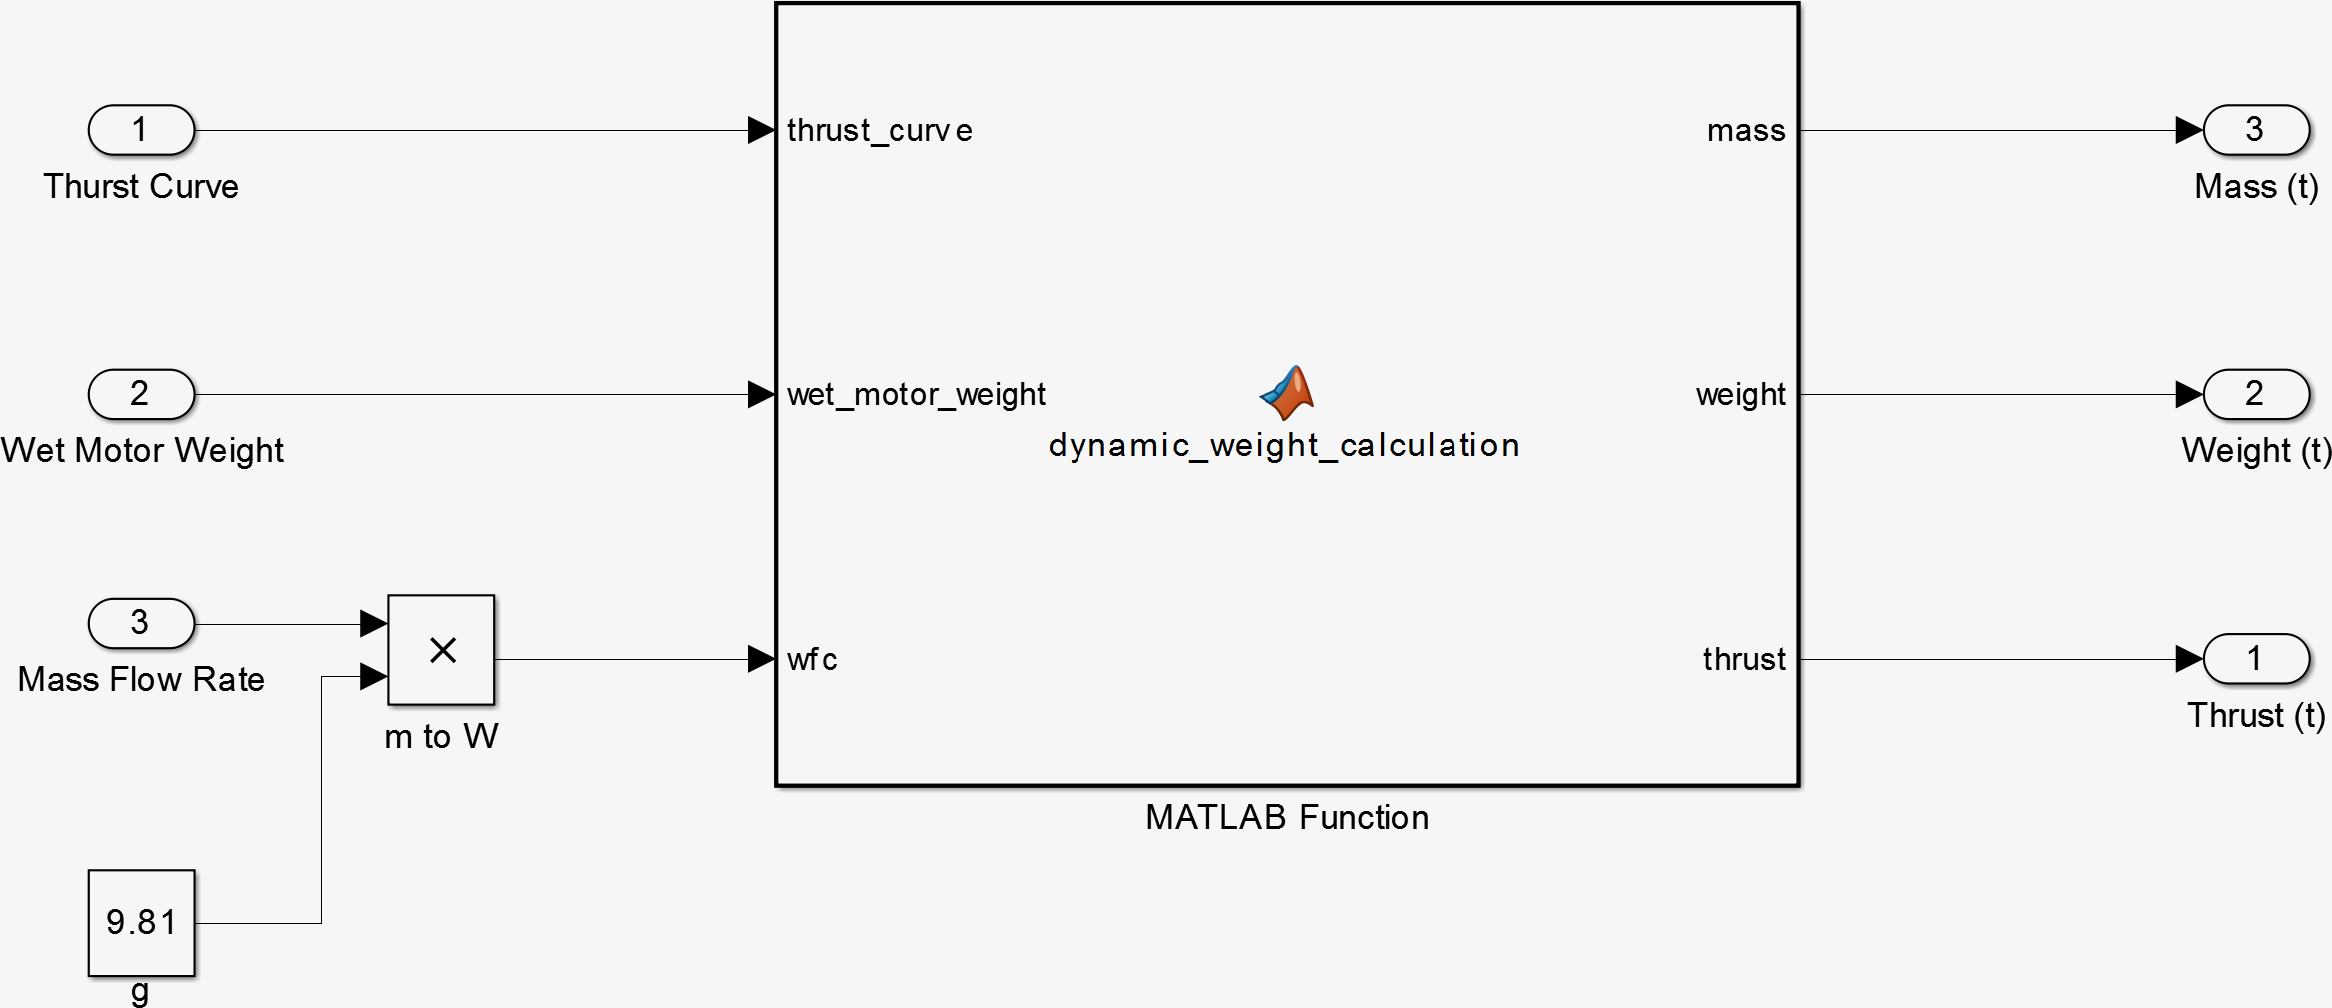
\includegraphics{images/dynamic_parameter_calculation.png}
\caption{Dynamic Parameter Calculation
\label{dynamic_parameter_calculation_label}}
\end{figure}

\begin{verbatim}
function [mass, weight, thrust] = dynamic_weight_calculation(thrust_curve, wet_motor_weight, wfc)
%------------------------------------------------------------------------------
% INPUT PARAMETERS
% thrust_curve     - a horizontal data set containing time and thrust
%                    data from a given motor    
% wfc              - the rate of motor weight loss due to fuel consumption 
% wet_motor_weight - the weight in Newtons of a motor *including* 
%                    propellant
%
% NOTE: this implementation skips the W_dot evaluation, just uses mfc 
% NOTE: UNTESTED
%------------------------------------------------------------------------------

% create the weight curve from an input thrust curvve matlab file 
% with the same dimensions as the input thrust curve
% weight_curve = {'time','weight'}

% grab the size of the input thrust curve
data_length = size(thrust_curve,1);

% create the corresponding weight curve, same size
weight = zeros(data_length,1);
    
%for i = 1:length(thrust_curve)
for i = 1:data_length
    weight(i,1) = wet_motor_weight - wfc*thrust_curve(i,1); 
end

thrust = thrust_curve;
mass = weight * 9.81;
\end{verbatim}

\subparagraph{Unit Testing}\label{unit-testing}

\begin{verbatim}
%------------------------------------------------------------------------------
%
% Dynamic Weight Calculation Test
%
% run the function against input thrust data
%------------------------------------------------------------------------------

g                = 9.81;
wet_motor_weight = 5.906*g;
dry_motor_weight = 3.624*g;
mfc              = 0.8236*g;

thrust_curve = thrust_data_import('monotomic_time_thrust_curve.csv');

burntime     = thrust_curve(:,1);
thrust_force = thrust_curve(:,2);

subplot(2,1,1);
plot(burntime,thrust_force);
title('Dynamic Weight Calculation Test - Motor Thrust Curve');
ylabel('Thrust - T (N)');
xlabel('Time - t (s)');

[actual_mass, actual_weight, actual_thrust] = dynamic_weight_calculation(thrust_curve, wet_motor_weight, mfc);

subplot(2,1,2);
plot(burntime,actual_weight(:,1))
title('Dynamic Weight Calculation Test - Motor Weight Curve');
ylabel('Weight - W (N)');
xlabel('Time - t (s)');

% TODO need to provide some hand-calculated data to assert against

% check that the last weight value is equal to the dry motor weight
%assert ( actual_weight_curve(122,1) == dry_motor_weight );
last_row = size(actual_weight,1);
final_weight = actual_weight(last_row, 1);

% TODO right now this assertion fails because the thrust data is not interpolated
assert ( dry_motor_weight == final_weight );
\end{verbatim}

The following figure shows the output of the test. The Thrust and Weight
curves are output as expected.

\begin{figure}[htbp]
\centering
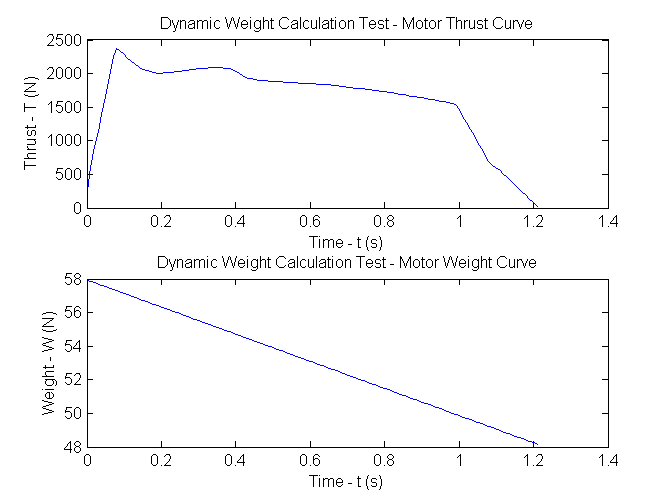
\includegraphics{images/dynamic_weight_calculation_test_figure.png}
\caption{Dynamic Weight Calculation Test Output
\label{dynamic_weight_calculation_test_figure_label}}
\end{figure}

\subsubsection{Center of Pressure}\label{center-of-pressure}

The \emph{Center of Pressure} (COP) is the location where the
aerodynamic forces are said to be acting. A wind tunnel is the best way
to approximate this point, but an analytic method is available.

\begin{equation}
\label{rocket_center_of_pressure}
\bar{X} = 
\dfrac
{ \left( C_{N \alpha} \right)_n \bar{x}_n + \left( C_{N \alpha} \right)_{cs} \bar{x}_{cs} + \left( C_{N \alpha} \right)_{cb} \bar{x}_{cb} + \left( C_{N \alpha} \right)_{fb} \bar{x}_{fb} }
{ C_{N \alpha}  }
\end{equation}

{[}4{]}

\paragraph{Barrowman's Equations}\label{barrowmans-equations}

\emph{Barrowman's Equations} are used to determine the center of
pressure.

\subsubsection{Center of Gravity}\label{center-of-gravity}

\begin{equation}
y_{cg} = \dfrac{m_1 y_1 + m_2 y_2 + ... + m_n y_n}{\sum_{j=1}^n m_j}
\end{equation}

\begin{equation}
COG(t) = \dfrac{m_1 y_1 + (m_2 - \Delta m) y_2}{m_1 + m_2 - \Delta m(t)} 
\end{equation}

Where COG(t) is the Center of Gravity as a function of time, \(m_1\) is
the static mass (combination of nose cone, body tube, and fins), \(m_2\)
is the initial mass of the motor, and \(\Delta m(t)\) is the change of
mass as a function of time due to fuel expenditure.

We consider the motor as a point mass centered at the geometric center
of the motor casing. This simplifies the calculation of the center of
gravity of the rocket as fuel is expended, as only the mass of the motor
is changing, and not the location of its particular center of mass.

\subsubsection{Moments of Inertia}\label{moments-of-inertia}

The instantaneous moment of inertia is determined by relating the moment
of inertias of the static structure and the dynamic structure through
the parallel axis theorem evaluated at the total center of gravity
(COG).

The sum of moment of inertias evaluated through the parallel axis
theorem nets the total moment of inertia.

\begin{equation}
I_n = I_{cm(n)} + M_P d^2 
\end{equation}

\begin{equation}
I_T(t) = \sum I_n 
\end{equation}

Where \(I_T(t)\) is the total moment of inertia of the rocket as a
function of time, and \(I_n\) is the component vector (either static or
dynamic moment of inertia)

{[}1{]}

\subsubsection{Longitudinal Moment of
Inertia}\label{longitudinal-moment-of-inertia}

To the \emph{Moment of Inertia} related to the pitch/yaw of the rocket
is the \emph{Longitudinal Moment of Inertia}.

\begin{equation}
\label{longitudinal_moment_inertia}
I = \dfrac{mL^2}{12}
\end{equation}

{[}TODO source dynamics textbook{]}

In keeping with the assumption of the motor as a point mass in the
volumetric center of the motor casing, the dynamic \emph{Longitudinal
Moment of Inertia} is calculated as follows.

\begin{equation}
\label{static_longitudinal_moment_inertia}
I_{static} + m_{static} r_{0 \rightarrow 1}^2
\end{equation}

Where \(r_{0 \rightarrow 1}\) is the distance between the static center
of gravity (the COG of the nose cone, body tube, and fins) and the
instantaneous center of gravity of the rocket. \(I_{static}\) is
provided by CATIA.

\begin{equation}
\label{motor_longitudinal_moment_inertia}
I_{motor} = \dfrac{m_{motor}L_{motor}}{12} + m_{motor}r_{0 \rightarrow 2}^2
\end{equation}

Where \(L_{motor}\) is the length of the motor casing, and
\(r_{0 \rightarrow 2}\) is the distance between the motor center of
gravity and the rocket center of gravity.

Then, the rocket \emph{Longitudinal Moment of Inertia} is the sum, shown
as follows

\begin{equation}
\label{rocket_longitudinal_moment_inertia}
I_{rocket} = I_{motor} + I_{static}
\end{equation}

\section{\texorpdfstring{Vertical (AOA \textless{} 5\(^\circ\)) Flight
Model}{Vertical (AOA \textless{} 5\^{}\textbackslash{}circ) Flight Model}}\label{vertical-aoa-5circ-flight-model}

\subsection{Particular Assumptions}\label{particular-assumptions}

The rocket is to be launched on a guide that may have a \(\pm\)
5\(^\circ\) angle. Considering the small angle approximation, the sine
of 5 degrees or less is approximately equal to the angle in radians, or
zero.

For a 1\% error: (@) \[ sin ( \theta \le 15^\circ ) \approx 0 \]
\href{http://www.physics.umanitoba.ca/undergraduate/phys2260/Lectures/Intro\%20Optics\%20-\%20PPT\%20v1part\%2004.pdf}{UManitoba}

This assumption greatly simplifies the simulation analysis. We consider
that the rocket flies perfectly vertical (experiencing no significant
drift) into still (quiescent) air for which density is described by the
\href{https://en.wikipedia.org/wiki/International_Standard_Atmosphere}{International
Standard Atmosphere (ISA) model}.

\subsection{Simplified Model}\label{simplified-model}

The dynamics of the rocket flights can be simplified to a sum of forces.

Simplifying the rocket flight as ideally one-dimensional, with the
positive x direction being upwards from the launch pad, the impulse is
equal to the thrust of the rocket minus the weight of the rocket and the
drag forces of the rocket interacting with the surrounding air.

\begin{equation}
m(t)\ddot{x}(t) = T(t) - D(\dot{x}) - W(t)
\end{equation}

Mass is a function of time, which is explained in the \emph{Dynamic
Parameters} section. Drag is a function of velocity, which is explained
in \emph{Drag Model} section. Acceleration can be expressed as the first
derivative of velocity and also the second derivative of position, each
with respect to time.

\begin{equation}
\vec{a} = \dot{v} = \ddot{x}
\end{equation}

Each force component can be rearranged and expressed as follows:

\begin{equation}
\vec{a}_T = \dfrac{T(t)}{m(t)}, \vec{a}_W = \dfrac{W(t)}{m(t)}, \vec{a}_D = \dfrac{D(v)}{m(t)}
\end{equation}

The net upward acceleration is: \(\vec{a}_T - \vec{a}_W - \vec{a}_D\)

The sum of forces can be rearranged and acceleration can be solved for:

\begin{equation}
\label{vertical_flight_equation}
\vec{a} =  \ddot{x} = \dfrac{1}{m(t)} (T(t) - D(\dot{x}) - W(t)) 
\end{equation}

Acceleration can be integrated to find position and velocity.

\begin{equation}
\vec{v} = \int \vec{a} dx
\end{equation}

\begin{equation}
x = \iint \vec{a} dx
\end{equation}

Integration of equation (\ref{vertical_flight_equation}) in the model is
represented by the \(\dfrac{1}{s}\) block. The model is pictured in
Figure \ref{vertical_model_simplified}.

\begin{figure}[htbp]
\centering
\includegraphics{images/vertical_model_simplified.png}
\caption{Vertical Flight Model - Simplified
\label{vertical_model_simplified}}
\end{figure}

\subsection{Aerodynamic Geometry}\label{aerodynamic-geometry}

\subsubsection{Overview}\label{overview-1}

Related to aerodynamic geometry of the rocket, the specific parameters
of interest are the following:

\begin{itemize}
\tightlist
\item
  Outer Diameter of Rocket (\emph{OD})
\item
  Total Length of Rocket (\emph{L})
\item
  Height of Nose Cone (\(h_n\))
\item
  Thickness of Fins
\item
  Number of Fins
\item
  Width of Fins
\item
  Surface Area of Nose
\end{itemize}

\subsubsection{Surface Roughness}\label{surface-roughness}

\emph{Surface Roughness} is the deviation in the normal direction from a
surface of its features. It contributes to \emph{Skin Friction Drag}

\subsubsection{Fineness Ratio}\label{fineness-ratio}

The \emph{Fineness Ratio} is the ratio of the length to the outer
diameter

\begin{equation} 
f_B = \dfrac{L} {OD}
\end{equation}

\subsubsection{Fins}\label{fins}

\subsubsection{Aerodynamic Chord Length of
Fins}\label{aerodynamic-chord-length-of-fins}

Since there is no airfoil on the fin design, the \emph{Aerodynamic Chord
Length of the Fins} (\(L_{cf}\)) is equal to the height of the fins.

\subsubsection{Areas}\label{areas}

Reference areas are required to calculate the drag force.

\paragraph{Wetted Body Area}\label{wetted-body-area}

The \emph{Wetted Body Area} is the combined area of all surfaces in
contact with moving air.

\paragraph{Frontal Reference Area}\label{frontal-reference-area}

The \emph{Frontal Reference Area} is the projected area of the rocket
perpendicular to the direction of air flow. For perfectly vertical
flight and quiescent air conditions, this is the precise projection of
the tip face of the rocket.

{[}TODO show figure{]}

\paragraph{Planform Area}\label{planform-area}

\subsection{Nose Profile}\label{nose-profile}

\subsubsection{Von Karman (Haack)}\label{von-karman-haack}

A \emph{Von Karman} nose profile has been selected by the design team,
other profiles will not be supported in the initial version of the
model. The \emph{Von Karman} nose profile is a \emph{Haack Series}
geometry, designed to minimize theoretical pressure drag
{[}niskanen2013{]}. This profile excels in subsonic flow conditions, and
performs well in transonic flow conditions {[}nassaNoseCone{]} - as such
is it well suited for the current mission.

The equation for the \emph{Haack Series} is

\begin{equation}
r(x) = \dfrac{R}{\sqrt{\pi}} \sqrt{ \theta - \dfrac{1}{2} sin (2 \theta) + \kappa \sin^3 \theta }
\end{equation}

Where

\begin{equation}
\theta = \cos^{-1} \left( 1 - \dfrac{2x}{L} \right)
\end{equation}

\href{http://rimworld.com/nassarocketry/fabrication/nosecones/design.html}{Nose
Profile Design}

\href{https://en.wikipedia.org/wiki/Nose_cone_design\#Von_K.C3.A1rm.C3.A1n}{Nose
Profile Design}

\subsection{Drag Model}\label{drag-model}

Rockets in flight experience multiple sources of drag. The total drag
effect is the sum of all specific drag effects.

Figure \ref{rocket_drag_sources_label} depicts the types of drag forces
to be expected in subsonic flight.

\begin{figure}[htbp]
\centering
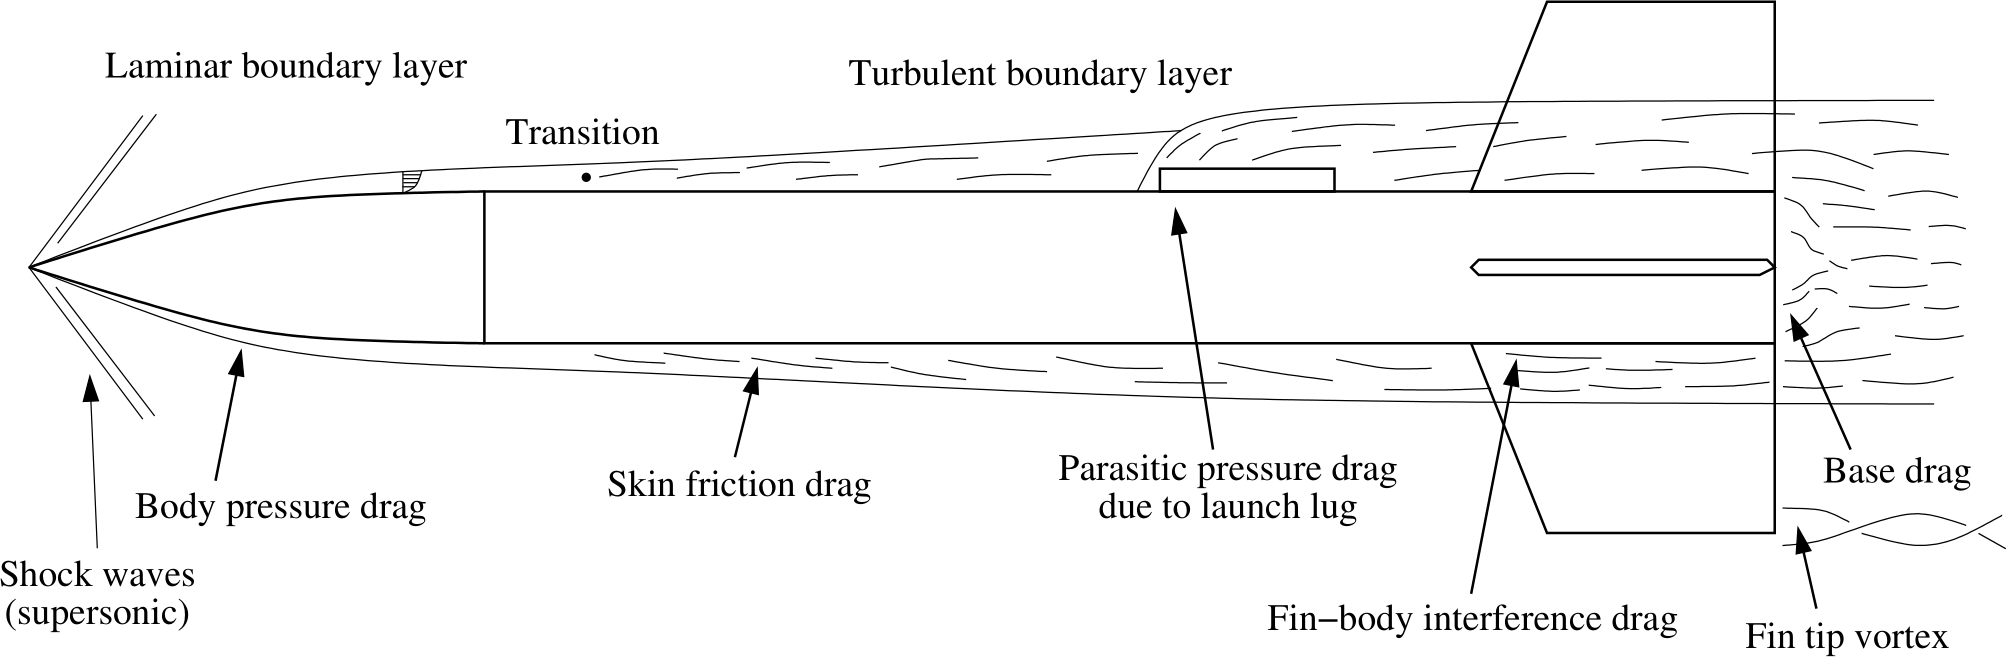
\includegraphics{images/drag_sources_niskanen2013.png}
\caption{Rocket Drag Sources - Subsonic Flight
\label{rocket_drag_sources_label}}
\end{figure}

{[}2{]}

The two main contributing factors to \emph{Drag Force} are \emph{Skin
Friction} and pressure distribution effects. Pressure distribution
effect are broken down into body pressure and parasitic drag effects,
among others {[}2{]}. These and other drag forces are detailed in this
section.

The drag model must take the parametric design parameters and applicable
dynamics parameters (see \emph{Data Model}) to output the Drag Force and
combined drag coefficient.

\subsubsection{Mach Number}\label{mach-number}

\emph{Mach Number} (M) is the ratio of the airspeed to the speed of
sound for air at a given temperature

The speed of sound (c) is calculated as follows

\begin{equation}
c = \sqrt{\gamma R T } 
\end{equation}

The \emph{Ideal Gas Law} states that

\begin{equation}
\label{ideal_gas_law}
P = \rho R T
\end{equation}

We can simplify our lives by assuming the \emph{Ideal Gas Law} applies,
and use it to solve for \emph{RT} using pressure and density.
\[ RT = \dfrac{P}{\rho} \]

Thus we can calculate the speed of sound as follows

\begin{equation}
\label{speed_of_sound}
c = \sqrt{\gamma \dfrac{P}{\rho} } 
\end{equation}

Where \(p\) is the local pressure, \(\rho\) is the local density, and
\(\gamma\) is the \emph{adiabatic index}, known as the \emph{isentropic
explansion factor} - it is the ratio of the specific heats of a gas at
constant pressure and constant volume.

{[}5{]}

The \emph{Mach Number} is then the ratio of the air velocity to the
sound speed of the local air

\begin{equation}
M = \dfrac{ \vec{v} } { c }
\end{equation}

\paragraph{Mach Regions}\label{mach-regions}

\emph{Velocity regions} are defined, in which aerodynamic effects are
known to vary considerably. The following velocity regions are
established for further discussion.

\begin{longtable}[c]{@{}ll@{}}
\toprule
Mach Region (\emph{M}) & Classification\tabularnewline
\midrule
\endhead
0.3 \textless{} 0.8 & Subsonic\tabularnewline
0.8 \textless{} M \textless{} 1 & Transonic\tabularnewline
1 \textless{} M \textless{} \textasciitilde{}5 &
Supersonic\tabularnewline
M \textgreater{} \textasciitilde{}5 & Hypersonic\tabularnewline
\bottomrule
\end{longtable}

\captionof{table}{Mach Regions}

{[}2{]}

As the rocket is constrained not to exceed Mach 0.9, much of the flight
will be in the subsonic region, greatly simplifying much of the
analysis. However, transonic effects cannot be ignored when at a Mach
Number greater than 0.8.

\subsubsection{Incompressible Flow}\label{incompressible-flow}

For Mach \textless{} 0.3,

\begin{quote}
In the incompressible flow regime the forces can be divided into
pressure force and viscous force
\end{quote}

\emph{Pressure Force} is due to fluid stagnation on areas of the rocket,
as well as due to the low pressure region created beyond the rocket at
is passes quickly through the air.

\emph{Viscous Force} is due to boundary layer effects and interactions
of moving air with surfaces. These forces are highly dependent on
Reynolds number. {[}1{]}

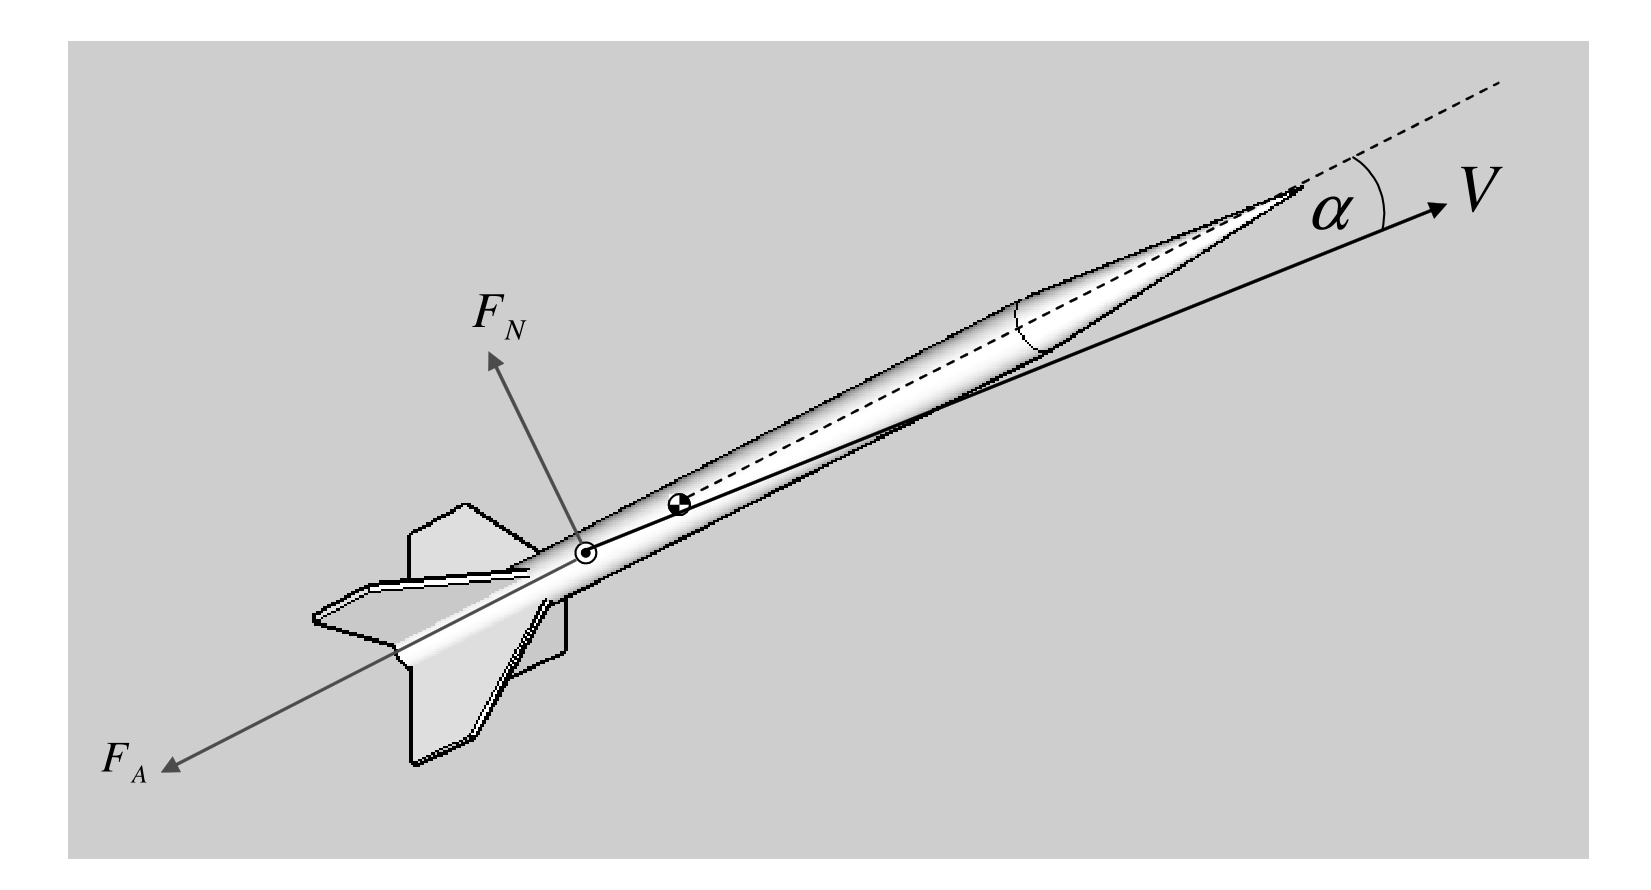
\includegraphics{images/rocket_drag_forces.png} {[}1{]}

Velocity \(\vec{v}\) is the apparent velocity of the center of pressure
relative to the surrounding air.

\subsubsection{Compressible Flow
Correction}\label{compressible-flow-correction}

Special considerations apply when compressibility effects are in play.
These effects occur above Mach 0.3 {[}1{]}, which will be easily
exceeded by the transonic upper limit of Mach 0.9 mandated by the
competition.

\begin{quote}
At low speeds (incompressible flow), the aerodynamic coefficients are
functions of the angle of attack (\(\alpha\)) and Reynolds number (Re).
\end{quote}

\begin{equation}
C_i (M < 0.3) = C_i (\alpha, Re) 
\end{equation}

\begin{quote}
At higher speeds (compressible, Ma \(\ge\) 0.4) they are also a function
of Mach number.
\end{quote}

\begin{equation}
C_i (M \ge 0.3) = C_i (\alpha, Re, M)
\end{equation}

Particular correction factors are recommended for ranges of Mach number

\begin{longtable}[c]{@{}ll@{}}
\toprule
Mach Number & Correction Factor\tabularnewline
\midrule
\endhead
\( M < 0.3 \) & N/A\tabularnewline
\( 0.3 < M < 0.8 \) &
\( C^`_i = \dfrac{C_i}{\sqrt{1-M^2}} \)\tabularnewline
\( 0.8 < M < 1.1 \) &
\( C^`_i = \dfrac{C_i}{\sqrt{1-(0.8)^2}} \)\tabularnewline
\( M > 1.1 \) & \( C^`_i = \dfrac{C_i}{\sqrt{M^2-1}} \)\tabularnewline
\bottomrule
\end{longtable}

\captionof{table}{Prandtl-Glauert Compressible Flow Correction Factors}

Where \(C_i\) is the incompressible drag coefficient and \(C^`_i\) is
the compressibility corrected drag coefficient {[}1{]}.

\subsubsection{Turbulent Effects}\label{turbulent-effects}

\begin{quote}
A turbulent boundary layer induces a notably larger skin friction drag
than a laminar boundary layer
\end{quote}

{[}2{]}

\subsubsection{Stagnation Pressure}\label{stagnation-pressure}

\emph{Stagnation Pressure} is the pressure on the normal surfaces to
airflow.

For a cylindrical rocket, it can be approximated as follows {[}2{]}

\begin{equation}
\label{eq_stagnation_pressure_blunt_cylinder}
\dfrac{q_{stag}}{q} =  
\begin{cases}
    1 + \dfrac{M^2}{4} + \dfrac{M^4}{40}                                    & M < 1 \\
    1.84 - \dfrac{0.76}{M^2} + \dfrac{0.166}{M^4} + \dfrac{0.035}{M^6}      & M > 1
\end{cases}
\end{equation}

Where \(q_{stag}\) is and \(q\) is

Then, the \emph{Pressure Drag Coefficient} can be expressed as a
function of \emph{Mach Number}

\begin{equation}
\label{eq_pressure_drag_coefficient}
C_{pr} = 0.85 \dfrac{q_{stag}}{q}
\end{equation}

\subsubsection{Reynolds Number}\label{reynolds-number}

The \emph{Reynolds Number} is a dimensionless number which describes the
ratio of the kinematic effects of a fluid to viscous effects.

\begin{equation}
\label{eq_reynolds_number_theory}
Re = \dfrac{\rho \vec{v} d}{\mu}
\end{equation}

{[}5{]}

\paragraph{Critical Reynolds Number}\label{critical-reynolds-number}

The \emph{Critical Reynolds Number} (\(Re_{crit}\)) is the value of
\emph{Reynolds Number} where the flow changes from laminar to turbulent.
This is greatly dependent on the surface roughness {[}munson2013{]}.

{[}2{]} gives the \emph{Critical Reynolds Number} as

\begin{equation}
\label{eq_reynolds_number_critical}
R_{crit} = \dfrac{\vec{v} x} {\nu}
\end{equation}

Where:

\begin{itemize}
\tightlist
\item
  \(\vec{v}\) is the free stream air velocty
\item
  \(x\) is the distance along the body from the nose cone tip where
  turbulent flow begins
\item
  \(\nu\) is the kinematic viscosity of air
\end{itemize}

For \(Re_{crit} = 5 \times 10^5\)

\begin{itemize}
\tightlist
\item
  \(\nu = 1.5 \times 10^-5 m^2/s\)
\item
  \(v_0 = 100 m/s\)
\item
  \$x = 7 cm \$ from the nose tip, where turbulent flow begins
\end{itemize}

{[}2{]}

\href{http://arxiv.org/ftp/arxiv/papers/1007/1007.0810.pdf}{Trinh, Khanh
Tuoc} \href{fluids\%20textbook}{See Fluids Text book}

Surface roughness has a considerable influence on \emph{Critical
Reynolds Number}. It can be determined as follows.

\begin{equation}
\label{eq_reynolds_number_critical_roughness}
R_{crit} = 51 \left( \dfrac{R_s}{L} \right)^{-1.039}
\end{equation}

{[}2{]}

\paragraph{Actual Reynolds Number}\label{actual-reynolds-number}

The \emph{Actual Reynolds Number} can be expressed in the following
form:

\begin{equation}
Re = \dfrac{\vec{v} L}{\nu} 
\end{equation}

Where:

\begin{itemize}
\tightlist
\item
  \(\vec{v}\) is the free stream velocity
\item
  \(L\) is the length of the rocket
\item
  \(\nu\) is the kinematic viscosity of the air in free stream
\end{itemize}

\subsubsection{Drag Force and
Coefficients}\label{drag-force-and-coefficients}

The total drag force is a function of air velocity (relative to the
rocket body) drag coefficient, reference area, and air density.

\begin{equation} 
D_f = D_f (\vec{v}, C_d, A_{ref}, \rho) 
\end{equation}

The drag coefficient \(C_d\) is the sum of all component drag
coefficients

\begin{equation} 
C_d = \sum C_i = C_{pa} + C_{fo} + C_{pr} + C_{in} + C_{ba} + C_{sk} + C_{fp} + C_{wa} + C_{bt} 
\end{equation}

From Fluid Mechanics {[}source?{]}

\begin{equation}
D_f = \dfrac{1}{2} C_d A_{ref} \rho \vec{v}^2  
\end{equation}

\paragraph{Viscous Drag Effects}\label{viscous-drag-effects}

\subparagraph{Skin Friction Drag}\label{skin-friction-drag}

Skin Friction Drag is due to viscous effects during flight, and is
significantly influenced by surface roughness.

\begin{equation}
\label{friction_drag_force}
D_{sk} = \dfrac{1}{2} \rho \vec{v}^2 A_{wet} C_{sk}
\end{equation}

{[}5{]}

Where

\begin{equation}
\label{friction_drag_coefficient}
C_{sk}, (A_{wet}, M, \dfrac{\epsilon}{l} )
\end{equation}

\(\dfrac{\epsilon}{l}\) is the relative roughness of the surface

With the critical and actual Reynolds Numbers determined, the
\emph{Uncorrected Skin Friction Drag Coefficient} can now be
conditionally determined

\begin{equation}
\label{eq_skin_drag_coefficient_uncorrected}
C_{sk_{uncorrected}} = 
\begin{cases}
    0.0148                                    & Re < 10^4 \\
    \dfrac{1}{(1.5 \ln Re - 5.6)^2}            & 10^4 < Re < Re_{crit} \\
    0.032 \left( \dfrac{R_a}{L} \right)^{0.2} & Re > Re_{crit}
\end{cases}
\end{equation}

{[}2{]}

Two other sources describe the cases for Skin Friction Drag Coefficient
differently.

\begin{equation}
C_{sk_{uncorrected}} = 
\begin{cases}
    \dfrac{1.328}{\sqrt{Re}} & Re \le Re_{crit} \\
    \dfrac{0.074}{Re^{1/5}}  & 10^4 < Re < Re_{crit}
\end{cases}
\end{equation}

{[}1{]} and {[}6{]} agree on the above.

The \emph{Skin Drag Coefficient Corrected for Compressibility} is:

Conversely, Niskanen evaluates the corrected skin drag coefficient as
follows

\begin{equation}
\label{eq_skin_drag_coefficient_corrected}
C_{sk_{corrected}} = C_{sk_{uncorrected}} \times 
\begin{cases}
     ( 1- 0.1 M^2 )                          & \text{Subsonic} \\
     \left[ (1+0.15 M^2)^{0.58} \right]^{-1} & \text{Supersonic} \\
     ( 1 + 0.18 M^2 )^{-1}                   & \text{Roughness Limited}
\end{cases}
\end{equation}

Finally, the \emph{Normalized and Corrected Skin Friction Drag
Coefficient} is:

\begin{equation}
C_{sk} = \dfrac{ C_{sk,c} \left[ \left( 1+ \dfrac{1}{2 f_B} \right) \cdot A_{wb} + \left( 1 + \dfrac{2t_f}{L_{cf}}\cdot \right) A_{wf} \right] }{A_{ref}}
\end{equation}

Where \(f_b\) is the \emph{Fineness Ratio}, the ratio of the length of
the rocket divided by the outer diameter. \(L_{cf}\) is the aerodynamic
chord length of the fins, and \(t_f\) is the thickness of the fins

{[}2{]}

\begin{equation}
\label{eq_reynolds_critical}
Re_{crit} = 51 \left( \dfrac{R_a}{L} \right) ^{-1.039} 
\end{equation}

\paragraph{Pressure (Form/Profile)
Drag}\label{pressure-formprofile-drag}

This is the drag caused by the pressure exerted on the surface of an
object as it moves through a free stream {[}5{]}.

\begin{equation} 
C_{pr}, D_{pr} (A_{ref}, M) 
\end{equation}

\subparagraph{Body Drag}\label{body-drag}

\emph{Body Drag} is the drag on the rocket forebody (pressure drag?)

\begin{equation}
\label{body_drag_coefficient}
C_{fb} = \left[ 1 + \dfrac{60}{(l_{TR}/d_b)^3} + 0.0025 \dfrac{l_b}{d_b} \right] \left[ 2.7 \dfrac{l_n}{d_b} + 4 \dfrac{l_b}{d_b} 2 \left( 1 - \dfrac{d_d}{d_b} \right) \dfrac{l_c}{d_b} \right] \cdot C_{f(fb)}
\end{equation}

Where \(l_{TR}\) is the total length of the rocket body, \(l_c\) is the
length of the boat tail, \(d_b\) is the maximum body diameter and
\(d_d\) is the diameter of the rocket base. C f(fb) is the coefficient
of viscous friction on the rocket forebody (defined later in (45))

\subparagraph{Fin Pressure Drag}\label{fin-pressure-drag}

The \emph{Fin Pressure Drag} depends on the fin profile. The current
rocket will use a square (rectangular) profile, and can be determined as
follows.

\begin{equation}
C_{fp}, D_{fp} (A_{ref}, M) 
\end{equation}

Leading Edge pressure drag

\begin{equation}
    C_{D,LE} = C_{D,stag} = 0.85 \dfrac{q_{stag}}{q}
\end{equation}

The \emph{Body Base Drag Coefficient} is

\begin{equation}
C_{base} =
\begin{cases}
    0.12 + 0.13 M^2     &   M < 1 \\
    \dfrac{0.25}{M}     &   M > 1
\end{cases}
\end{equation}

For perpendicular orientation of the fin edges to air flow, the
stagnation pressure defined in Equation
\ref{eq_stagnation_pressure_blunt_cylinder} is used.

\[
\dfrac{q_{stag}}{q} =  
\begin{cases}
    1 + \dfrac{M^2}{4} + \dfrac{M^4}{40}                                    & M < 1 \\
    1.84 - \dfrac{0.76}{M^2} + \dfrac{0.166}{M^4} + \dfrac{0.035}{M^6}      & M > 1
\end{cases}
\] {[}2{]}

\subparagraph{Von Karman Nose Pressure
Drag}\label{von-karman-nose-pressure-drag}

Most nose cone shapes can be approximated to produce zero pressure drag
at subsonic velocities, however complications arise for transonic and
supersonic velocities. A semi-empirical method can be employed in the
latter conditions.

\begin{quote}
The curves of the pressure drag coefficient as a function of the nose
fineness ratio \(f_N\) can be closely fitted with a function of the form
\end{quote}

\begin{equation}
C_{d_pressure} = \dfrac{a}{(f_N + 1)^b}
\end{equation}

Where \emph{a} and \emph{b} are calculated from two data points
corresponding to fineness ratios 0 and 3

{\textbf{???}}

In subsonic and transonic regions, pressure drag of nose cones is
calculated as follows:

\begin{equation}
\begin{cases}
    0.8 \cdot \sin^2 \phi               & M \approx 0 \\
    a \cdot M^b + 0.8 \cdot \sin^2 \phi & M \approx 0.8
\end{cases}
\end{equation}

Where \emph{a} and \emph{b} are computed by interpolation to fit the
drag coefficient and the derivative of the drag coefficient at the lower
bound of the transonic region.

The cause of this drag is slight flow separation, and as such cannot be
corrected due to compressibility effects.

{[}2{]}

\subparagraph{Base Drag}\label{base-drag}

Base drag is caused by a low pressure region generated behind the base
of the rocket as it moves quickly through the atmosphere {[}2{]}.
Specifically, it is due to boundary separation between the flow past the
rocket and the surrounding air {[}1{]}. The flowing air attempts to make
a sharp turn around the sudden geometry change at the base end of the
rocket, however, viscous effects resist this change in direction. As a
result, pressure cannot be equalized in the space directly behind the
rocket and a low-pressure (vacuum) region forms {[}7{]}. This
low-pressure region has an effect analogous to \emph{pulling} the rocket
against its direction of flight.

\begin{equation}
C_{ba}, D_{ba} ((A_{ref}, M)) 
\end{equation}

\begin{equation}
\label{eq_base_drag_coefficient}
C_{ba} = 
\begin{cases}
0.12+0.13 M^2   & M < 1 \\
\dfrac{0.25}{M} & M > 1
\end{cases}
\end{equation}

{\textbf{???}}, pg.50

In reality, this low pressure region is disturbed by the thrust envelope
from the motor. Thus, we would expect base drag to be different during
the motor burn time than during the free flight after all fuel was
exhausted. Considering the thrust envelope is at this moment beyond the
scope of the project. Instead, an accepted approximation is to subtract
the area of the motor from the area of the base when calculating drag
force {[}2{]}.

\begin{equation}
\label{eq_base_drag_force}
D_{ba} = \dfrac{1}{2} C_{ba} \rho (A_{tube,base} - A_{motor,base}) \vec{v}^2 
\end{equation}

We can normalize the base drag coefficient to take this into account.

\begin{equation}
\label{eq_base_drag_coefficient_normalized}
C_{ba,normalized} =
C_{ba} * A_{tube,base}/A_{motor,base}
\end{equation}

\subparagraph{Shoulder Pressure Drag}\label{shoulder-pressure-drag}

The drag coefficient of the shoulder interfacing the body tube is
assumed to be equal to that of the body tube itself, and also assumes a
smooth interface. This is likely to be sufficient for subsonic velocites
{[}2{]}, and for the scope of this project it is neglected entirely.

\subparagraph{Parasitic Drag}\label{parasitic-drag}

Parasitic drag is the drag due to body features not explicitly designed
and/or imperfections not easily approximated. Examples include launch
guides, ventilation holes, surface roughness, and any damage during
flight.

PARASITIC DRAG IS CURRENTLY NEGLECTED IN THE MODEL, gt

\begin{equation}
C_{pa}, D_{pa} (A_{ref}, M) 
\end{equation}

Where \(C_{stag}\) is the \emph{Stagnation Drag Coefficient} {[}see
equation from fin pressure drag section{]}

We consider the most significant source of \emph{Parasitic Drag} to be
the launch lug. If there is no significant airflow through the launch
lug, we can approximate it as a cylinder next to the rocket body.
\emph{Niskanen} states that a launch lug with a length at least two
times its width has a drag coefficient of 0.74, with its reference area
being the frontal area. Stagnation pressure proportionally influences
the drag coefficient {[}2{]}.

The following equation relates the launch lug diameter \(\phi_{lug}\) to
the launch lug tube length \(l_{lug}\).

\begin{equation}
C_{pa} = \left( 1.3 - 0.3 \dfrac{l_{lug}}{\phi_{lug}} , 1 \right)_{max} \cdot C_{stagnation} 
\end{equation}

Where \emph{L} is the rocket length, \(h_n\) is the height of the nose
cone, \emph{OD} is the outer diameter of the rocket, and
\(C_{stagnation}\) is the stagnation coefficient {[}2{]}.

The reference area of the launch lug is given as follows

\begin{equation}
\label{eq_area_reference_launch_lug}
\pi \cdot (r_{ext,lug}^2 - r_{int,lug}^2) \cdot 
\left[ 1 - \left( \dfrac{l_{lug}}{\phi_{lug}} \right) \right]_{+ve} 
\end{equation}

The \emph{Parasitic Drag Coefficient} can be normalized to the reference
area of the launch lug.

\begin{equation}
\label{eq_coef_drag_parasitic_normalized}
C_{pa_{norm}} = 
C_{pa} \cdot 
\left( 
\pi \cdot (r_{ext}^2 - r_{int}^2) \cdot 
\left[ 1 - \left( \dfrac{L-h}{OD} \right)  \right]_{+ve} 
\right) 
\end{equation}

{[}2{]}

\begin{figure}[htbp]
\centering
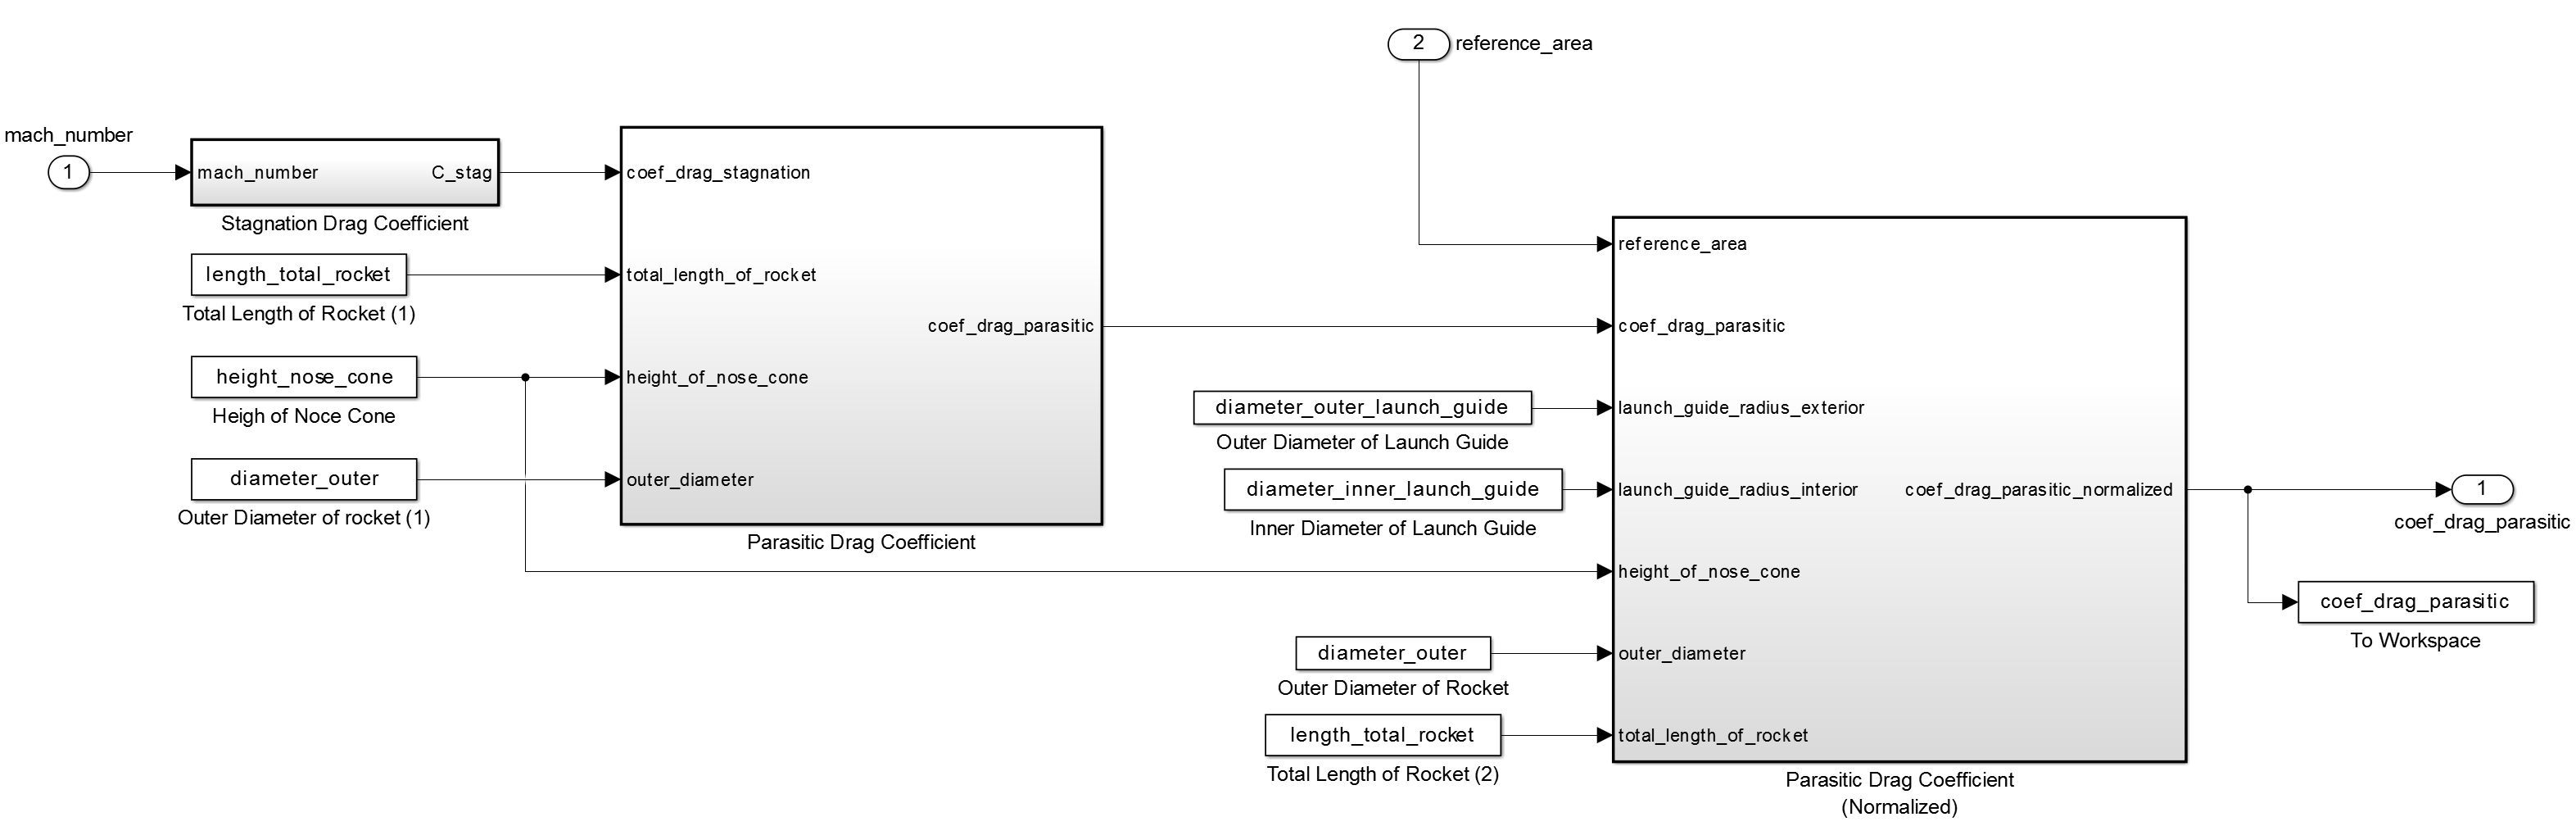
\includegraphics{images/drag/coef_drag_parasitic.png}
\caption{Matlab Implementation of Parasitic Drag
Coefficient\label{img_coef_drag_parasitic_label}}
\end{figure}

\subparagraph{Interference Drag}\label{interference-drag}

\emph{Interference Drag} is caused due to effects of air flow at the
interfaces of the fins and the body.

\begin{equation} 
C_{in}, D_{in} (A_{ref}, M) 
\end{equation}

\begin{equation}
\label{eq_interference_drag_coefficient}
C_{in} = 2 C_{sk,fins} \left( 1 + 2 \dfrac{T_f}{l_m} \right) \dfrac{4n(A_{f_p}-A_{f_e}} {\pi d^2_f}
\end{equation}

Where: - \(C_{sk,fins}\) is the coefficient of skin friction (due to
viscous effects) on the fins - \(n\) is the number of fins - \(A_{f_p}\)
is the fin planform area

\begin{equation}
\label{eq_fin_planform_area}
A_{f_p} = A_{f_e} + \dfrac{1}{2} d_f l_r
\end{equation}

\begin{itemize}
\tightlist
\item
  \(A_{f_e}\) is the exposed planform area of the fin

  \begin{equation}
  \label{eq_exposed_fin_planform_area}
  A_{f_e} = \dfrac{1}{2} (l_r + l_t) l_s 
  \end{equation}
\end{itemize}

{[}1{]}

Interference Drag effects are small in comparison to other drag effects
{[}2{]}, and are thus ignored at this stage of the project.

\paragraph{Wave Drag}\label{wave-drag}

\emph{Wave drag} is drag associated with shock waves (independent of
viscous effects).

\begin{quote}
At transonic speed, shock waves form at the nose tip and at the leading
edge of the fins \ldots{} Momentum is transferred from the rocket to the
surrounding air via these shockwaves
\end{quote}

\paragraph{Boat-Tail Drag}\label{boat-tail-drag}

A \emph{boat-tail} is a reduction in diameter of the body tube towards
the base of the rocket. Our rocket does not have a boat-tail, thus
\emph{Boat-Tail Drag} considerations are ignored.

\clearpage 

\subsubsection{Matlab Implementation}\label{matlab-implementation-1}

Figure \ref{rocket_drag_model_label} below shows the \emph{Simulink}
implementation of the calculation of the drag model

\begin{figure}[htbp]
\centering
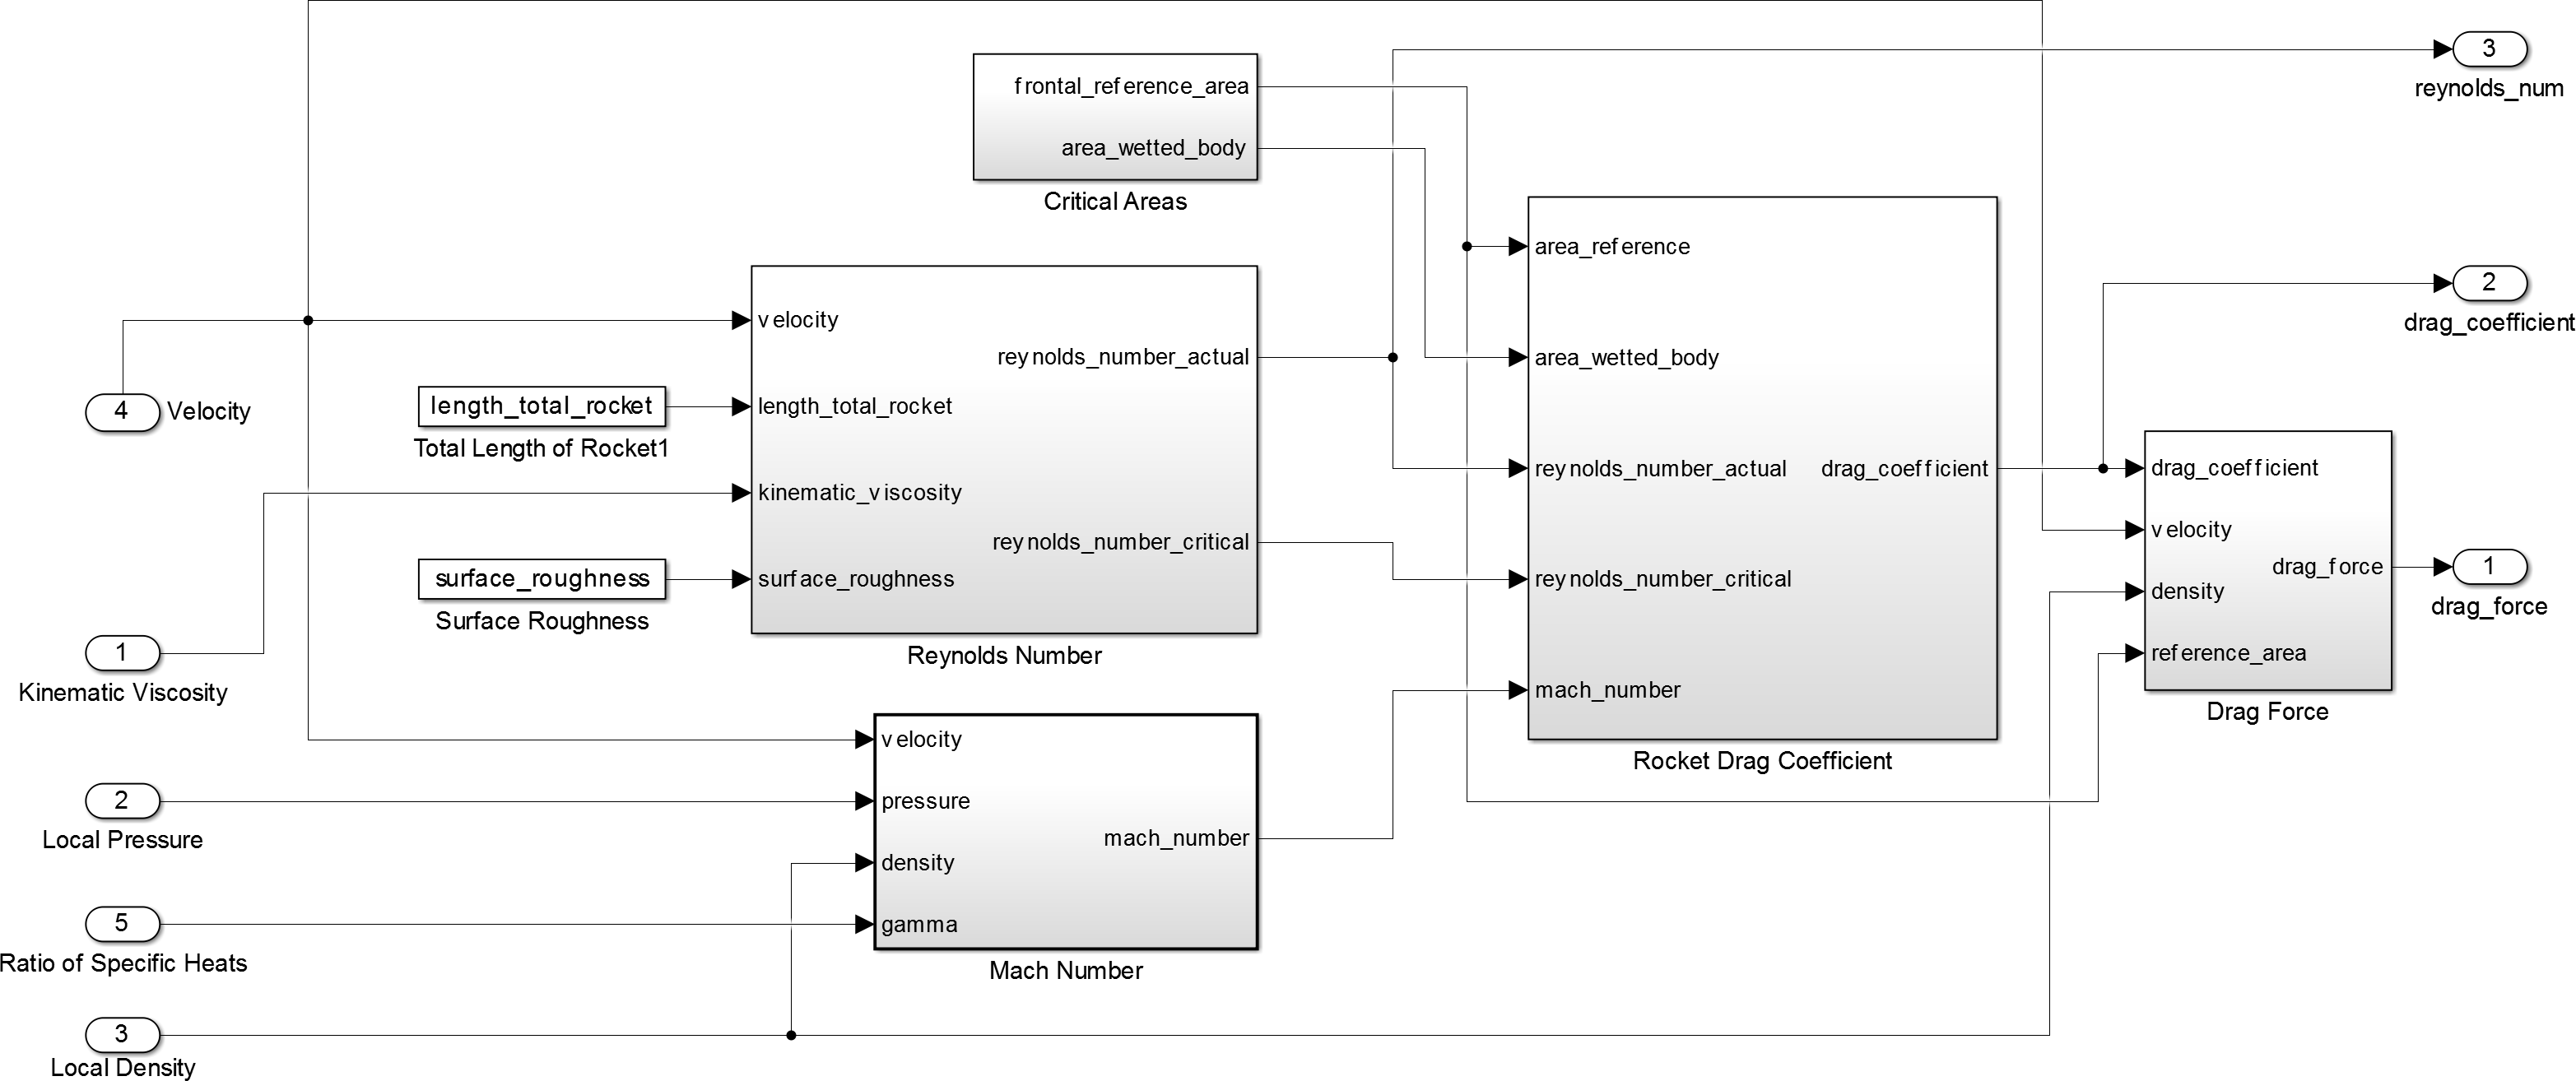
\includegraphics{images/rocket_drag_model.png}
\caption{Rocket Drag Model\label{rocket_drag_model_label}}
\end{figure}

\clearpage

Figure \ref{rocket_drag_coefficients_label} below shows the
\emph{Simulink} implementation of the calculation of drag coefficient

\begin{figure}[htbp]
\centering
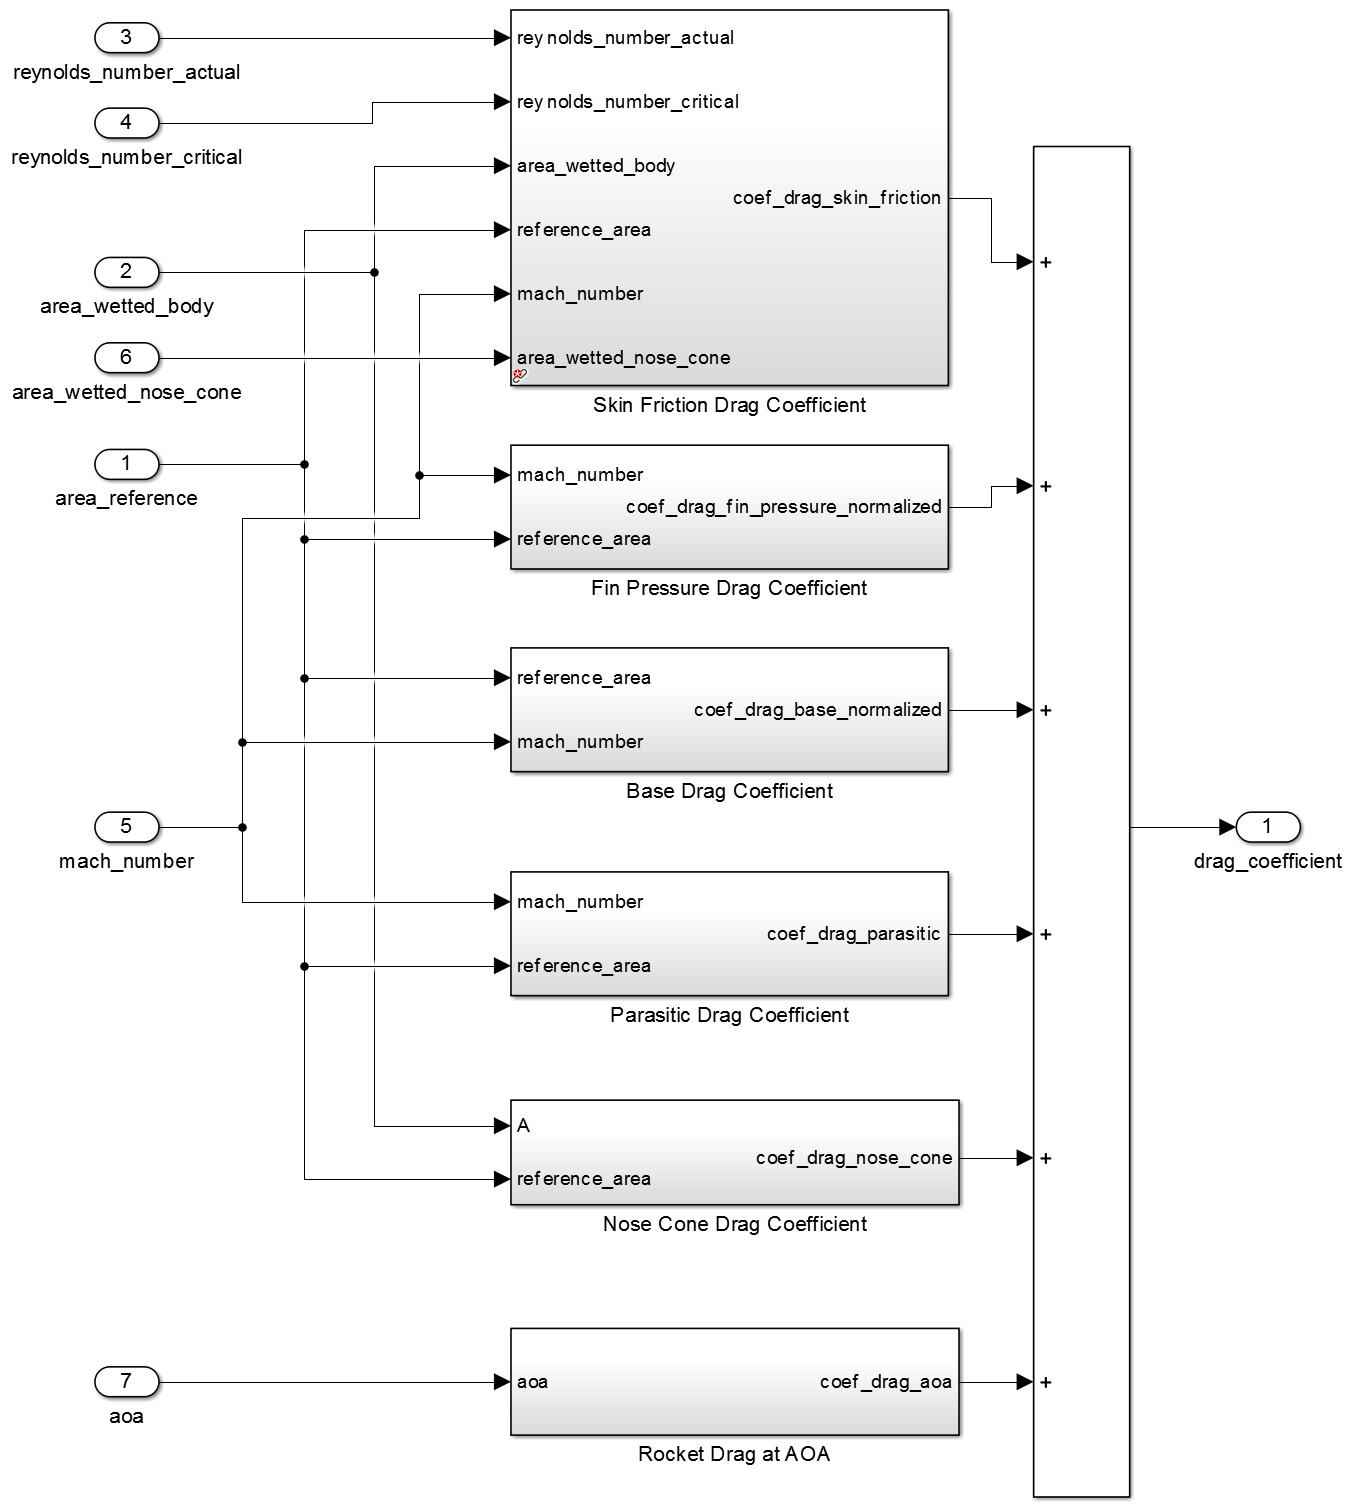
\includegraphics{images/rocket_drag_coefficient.png}
\caption{Rocket Drag Coefficient Model
\label{rocket_drag_coefficients_label}}
\end{figure}

\clearpage

\section{Angular Flight Stability (Pitch, Yaw)
Analysis}\label{angular-flight-stability-pitch-yaw-analysis}

\subsection{Overview}\label{overview-2}

\begin{itemize}
\tightlist
\item
  non-linear model (stability analysis)
\item
  finding lift will be annoying
\end{itemize}

\begin{quote}
``One of the first principles any rocket designer must learn is that a
rocket will fly only if the center of gravity is ahead of the center of
pressure far enough to allow the air currents to cause a stabilizing
effect.''
\end{quote}

http://www.nar.org/NARTS/TR13.html

\subsection{Out-of-scope}\label{out-of-scope}

\begin{itemize}
\tightlist
\item
  range (drift)
\item
  roll
\end{itemize}

\subsection{Requirement}\label{requirement}

\begin{itemize}
\tightlist
\item
  2a - The static stability margin falls above 2 (but less than 3)
  calibers at launch
\item
  2b - The dynamic stability is greater than 0 even in winds up to 8.33
  m/s
\item
  2f - The vehicle does not experience resonant pitching/yawing motion
  in flight
\end{itemize}

\subsection{Barrowman Method}\label{barrowman-method}

\subsubsection{Assumptions}\label{assumptions-2}

\begin{itemize}
\tightlist
\item
  incompressible flow
\item
  neglect viscous forces
\end{itemize}

{[}1{]}

\subsubsection{Rocket Normal Force}\label{rocket-normal-force}

\begin{equation}
\label{rocket_normal_force}
F_{N} = \dfrac{1}{2} \rho \vec{v}^2 A_{c} C_N
\end{equation}

{[}1{]}

Where \(A_c\) is the cross-sectional area of the body tube, and \(C_N\)
is the \emph{Normal Force Coefficient}, and is a function of
angle-of-attack (\(\alpha\))

\begin{equation}
\label{normal_force_coefficient}
C_N = C_{N \alpha} \cdot \alpha
\end{equation}

{[}1{]}

Where \(C_{N \alpha}\) is the \emph{Stability Derivative}, the slope of
the \emph{Normal Force Coefficient}. The total \emph{Stability
Derivative} is the sum of all rocket component stability derivatives

\begin{equation}
\label{total_stability_derivative}
C_{N \alpha} = \sum C_{N \alpha (P)}   
\end{equation}

{[}1{]}

\subsubsection{Compressibility
Correction}\label{compressibility-correction}

\emph{Barrowman's Method} neglects compressibility effects, however
these effects cannot be neglected above Mach 0.3.

\subsubsection{Rocket Body Lift
Correction}\label{rocket-body-lift-correction}

\emph{Barrowman's Method} neglects the lift generated by the rocket
body. Galejs {[}8{]} suggests the following adjustment to provide a
compensated \emph{Coefficient of Normal Force due to Body Lift}

\begin{equation}
\label{coefficient_normal_force_body_lift}
C_{N(L)} = K \dfrac{A_p}{A_{ref}} \alpha^2
\end{equation}

Where \(A_p\) is the \emph{planform area} of the rocket (the projected
length-wise area of the rocket, neglecting the fins)

\subsection{Longitudinal Static Stability
Margin}\label{longitudinal-static-stability-margin}

The \emph{Longitudinal Static Stability Margin} (\(S_{lm}\)) is the
distance between the \emph{Center of Gravity} and the \emph{Center of
Pressure} divided by the outer diameter of the body tube when the rocket
is positioned at an angle-of-attack (\(\alpha\)) of zero {[}TODO
source??{]}.

\[ S_{lm} = \dfrac{COP - COG}{OD} \]

The result is dimensionless, however the ratio determined is measured as
\emph{calibers}.

https://www.apogeerockets.com/education/downloads/Newsletter133.pdf

\subsection{Dynamic Stability}\label{dynamic-stability}

The rocket must exhibit dynamic stability, wherein oscillations are
reduced by the damping moment j

\subsubsection{Resonant Pitch/Yaw
Moment}\label{resonant-pitchyaw-moment}

\begin{itemize}
\tightlist
\item
  2f - The vehicle does not experience resonant pitching/yawing motion
  in flight
\end{itemize}

The rocket should experience a resonant motion in response to
aerodynamic forces such that it doesn't sustain at the natural
frequencies that can cause structural or component damage. This value
must be verified regularly with the design team to ensure compliance.

\subsubsection{Corrective Moment
Coefficient}\label{corrective-moment-coefficient}

\href{https://www.apogeerockets.com/education/downloads/Newsletter193.pdf}{Corrective
Moment Coefficient}

\subsubsection{Damping Moment
Coefficient}\label{damping-moment-coefficient}

\href{https://www.apogeerockets.com/education/downloads/Newsletter195.pdf}{Damping
Moment Coefficient - Source}

\subsection{Wind Impulse}\label{wind-impulse}

Two commonly used Wind Models are as follows

\subsubsection{Kaimal Wind Model}\label{kaimal-wind-model}

\begin{equation}
\label{eq_kaiman_wind_model}
\dfrac{S_u (f)}{\sigma ^2 _ u} = \dfrac{4 L_{1u} / U }{(1+6f L_{1u} / U )^{5/3}}
\end{equation}

\subsubsection{Von Karman Wind Model}\label{von-karman-wind-model}

\begin{equation}
\label{eq_von_karman_wind_model}
\dfrac{S_u (f)}{\sigma ^2 _ u} = \dfrac{4 L_{2u} / U }{(1+ 70.8 (fL_{2u} / U)^2 )^{5/3}}
\end{equation}

Where

\begin{itemize}
\tightlist
\item
  \(\dfrac{S_u (f)}{\sigma ^2 _ u}\) is the \emph{Spectral Density
  Function} of turbulence velocity
\item
  \emph{f} is the turbulence frequency
\item
  \(\sigma_u\) is the standard deviation fo the turbulence velocity
\item
  \(L_{1u}\) and \(L_{2u}\) are length parameters
\item
  \emph{U} is the average wind speed
\end{itemize}

{[}2{]}

\section{Validation}\label{validation-1}

\subsection{Integration Testing}\label{integration-testing}

\begin{figure}[htbp]
\centering
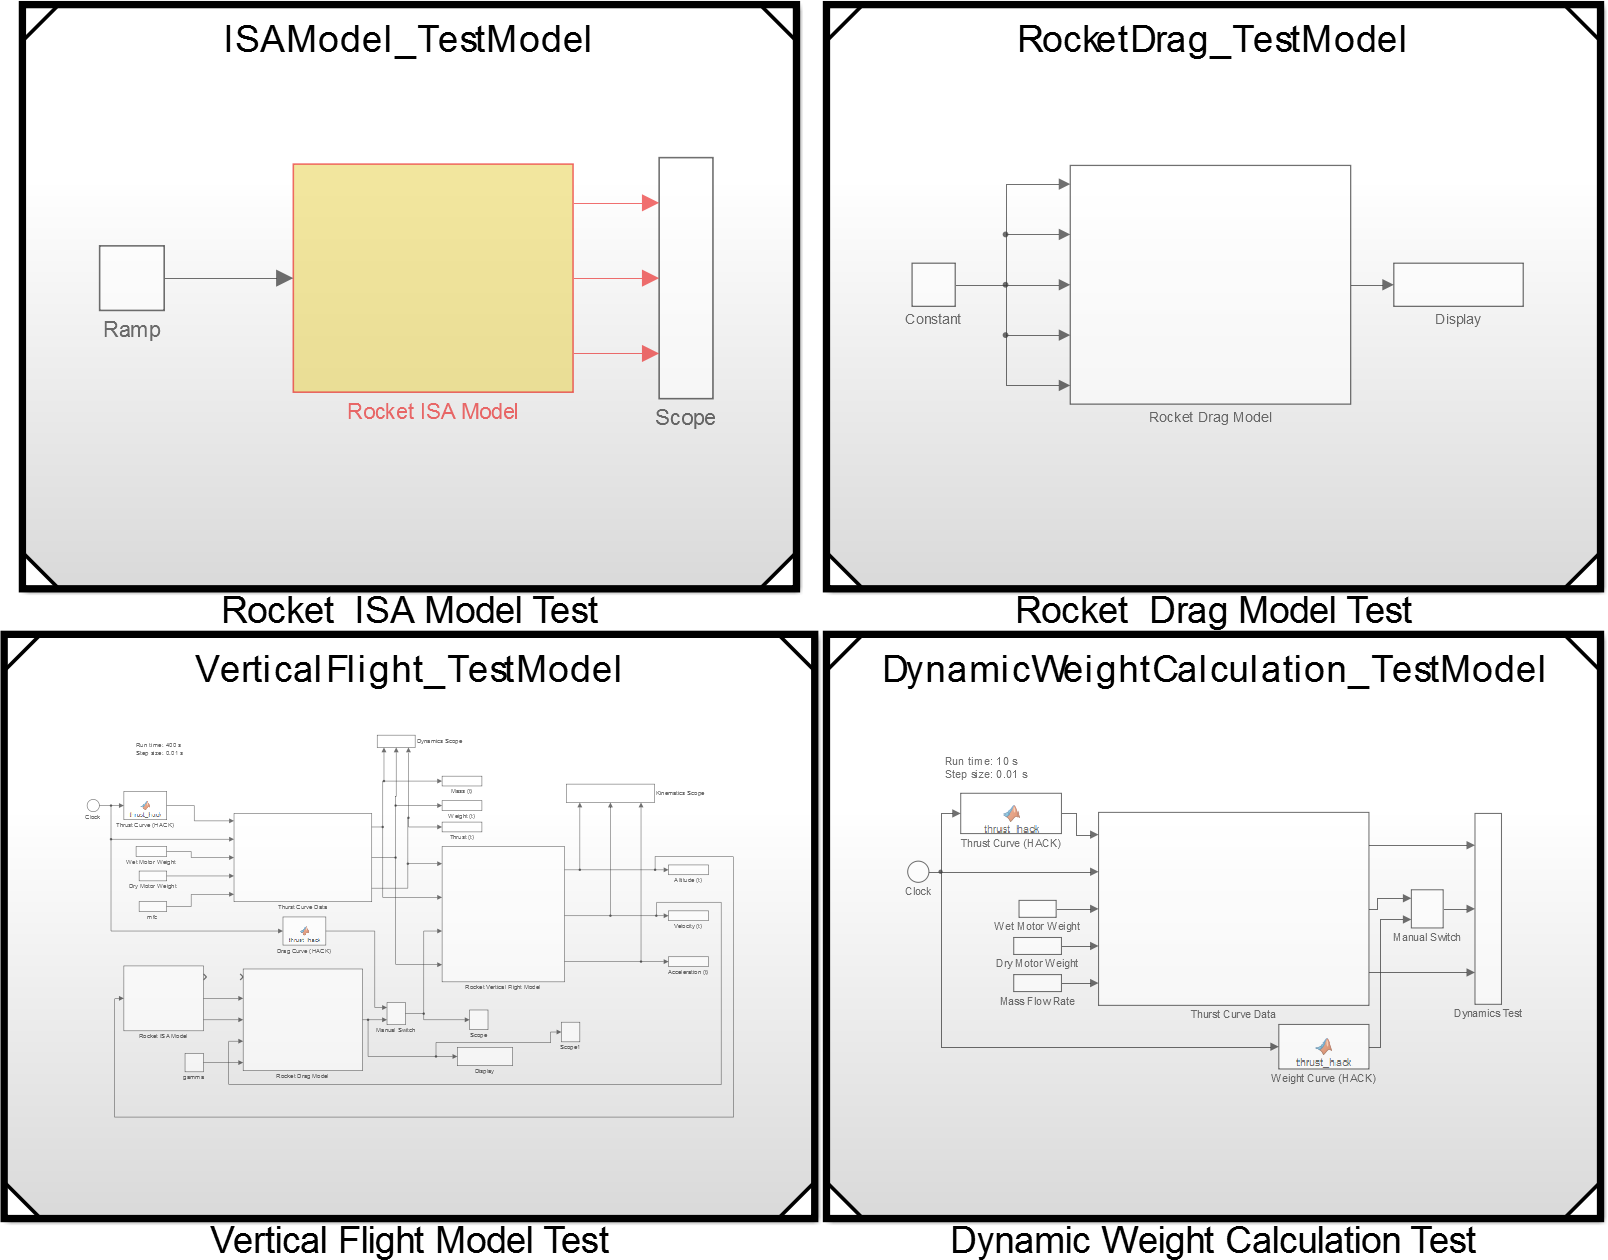
\includegraphics{images/ALL_TESTS.png}
\caption{All Integration Tests \label{all_integration_tests_label}}
\end{figure}

\clearpage

\section{Simulation Results}\label{simulation-results}

\subsection{Simulation Configuration}\label{simulation-configuration}

The following model was executed

\begin{figure}[htbp]
\centering
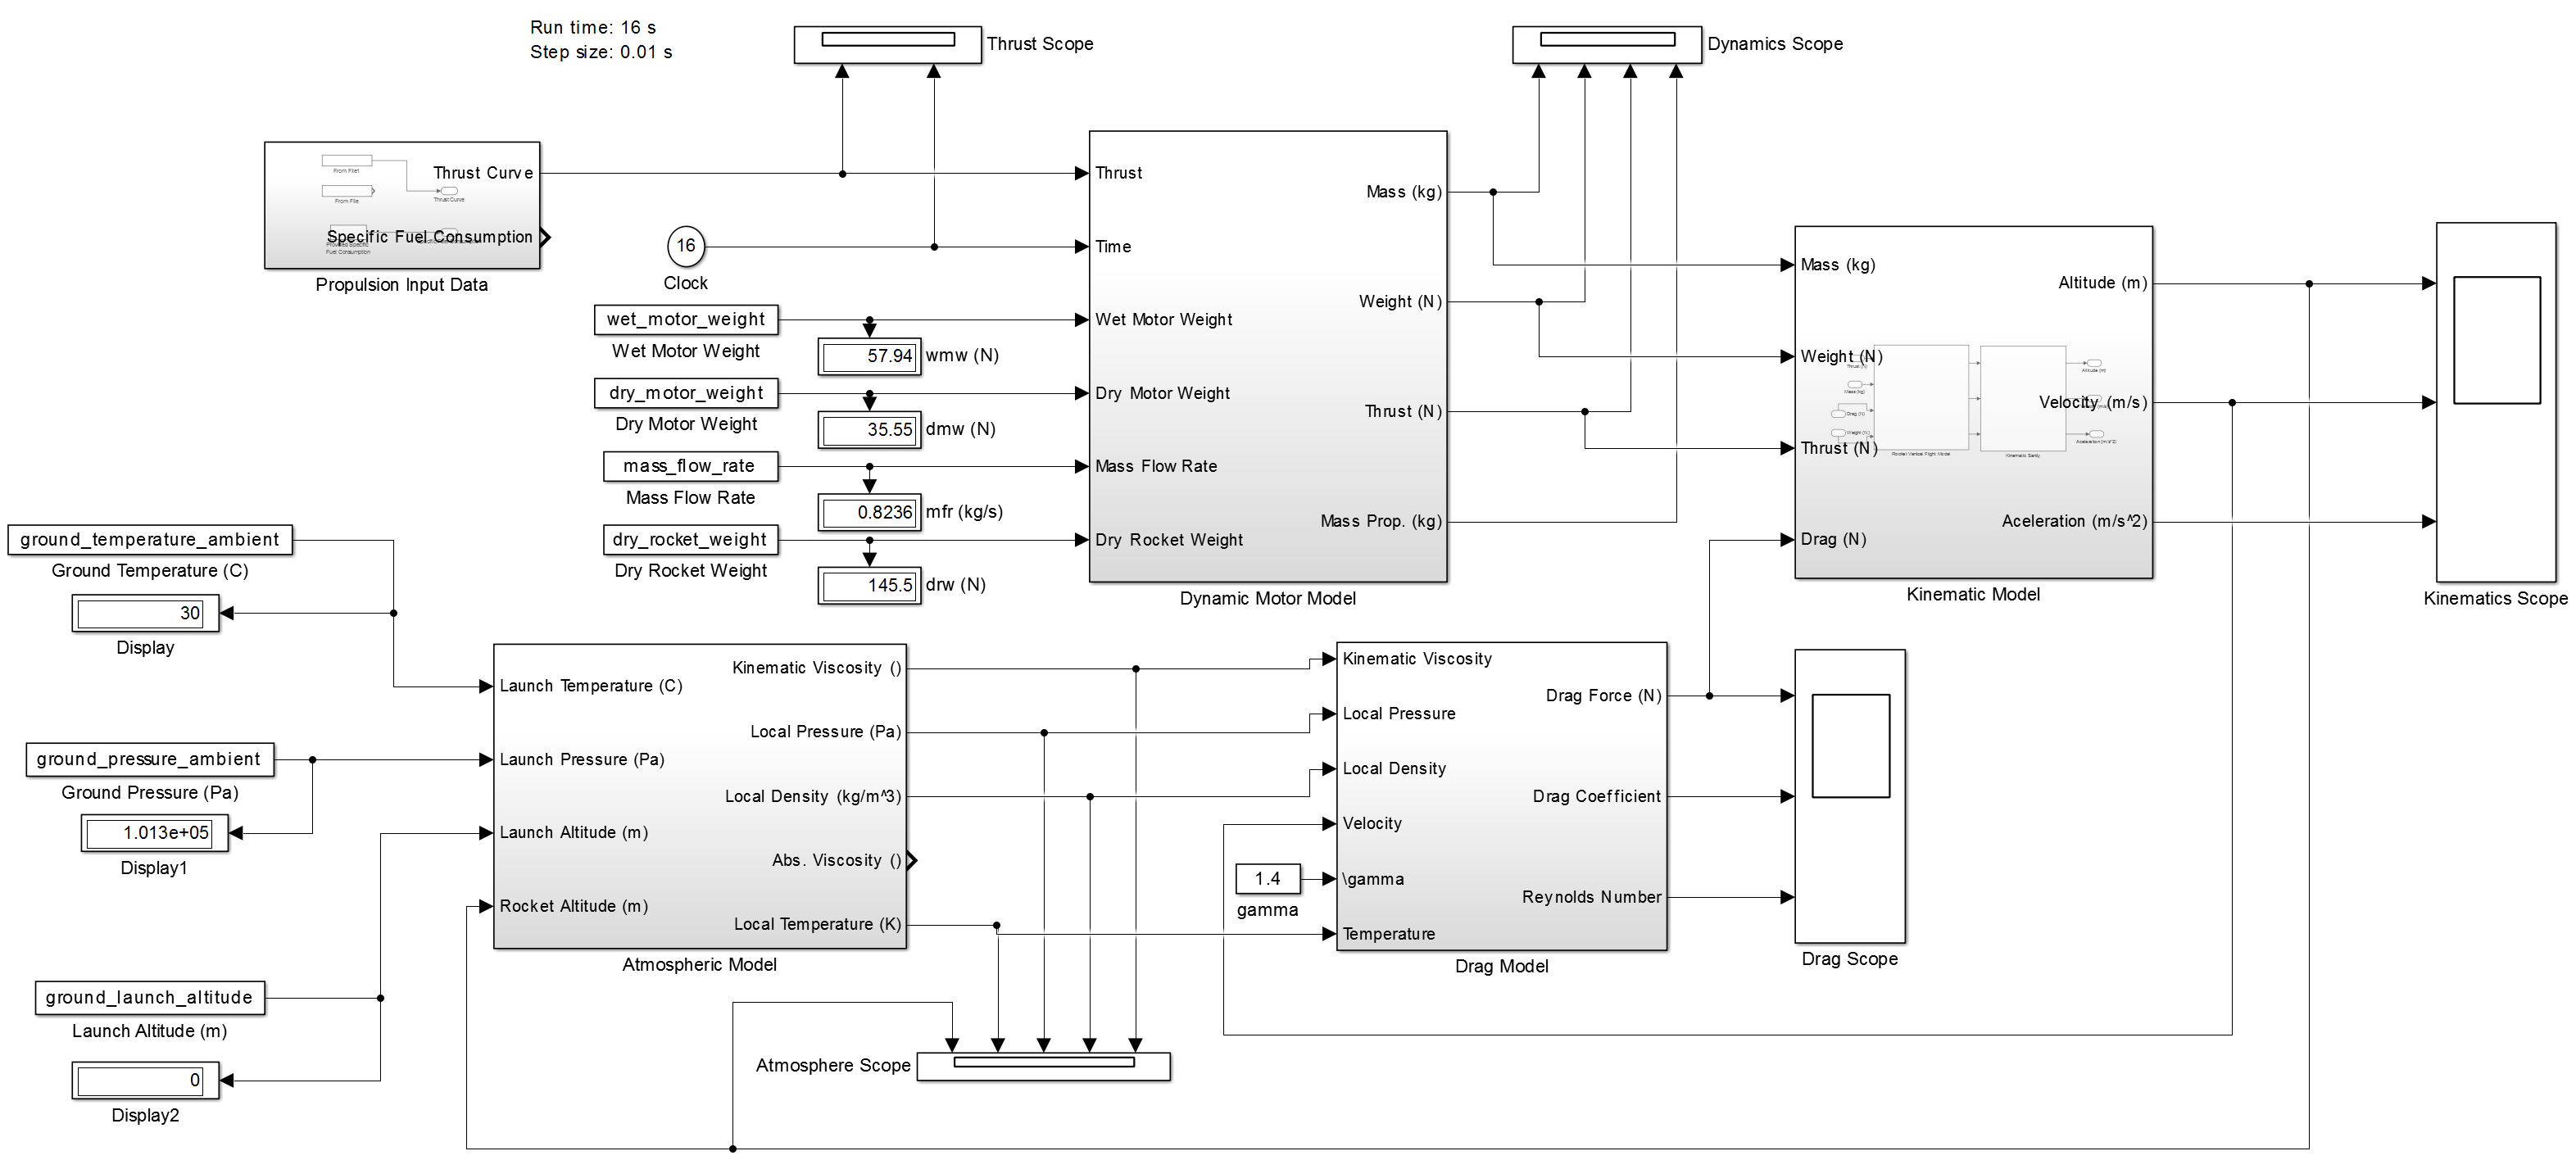
\includegraphics{images/vertical_model.png}
\caption{Vertical Model in Simulink, angle of attack less than 5 degrees
\label{vertical_model_test_label}}
\end{figure}

\subsection{Observations}\label{observations}

\subsection{Primary Plots}\label{primary-plots}

\begin{figure}[htbp]
\centering
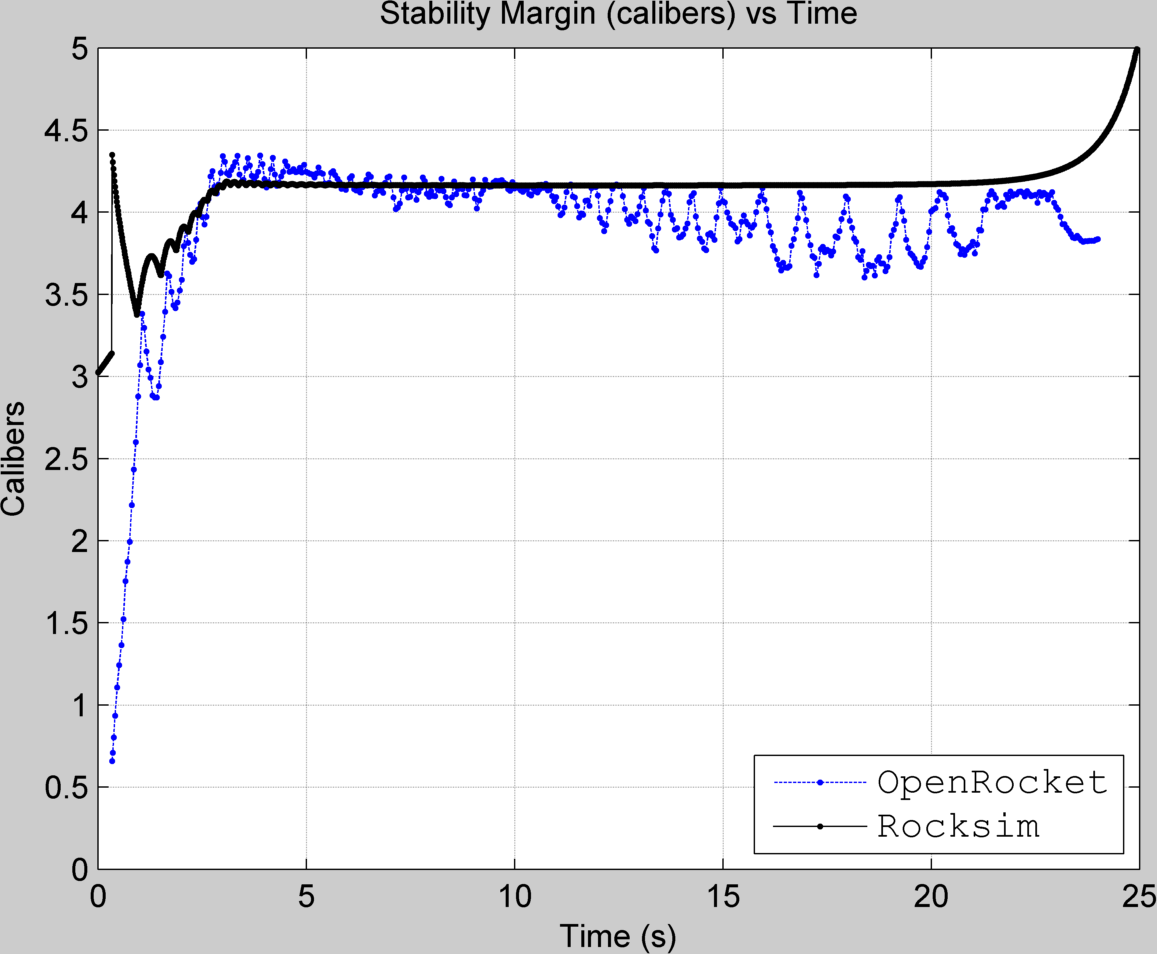
\includegraphics{images/plots/error_altitude_plot.png}
\caption{Mass, Weight, and Thrust as a Function of Time
\label{error_altitude_plot_label}}
\end{figure}

\begin{figure}[htbp]
\centering
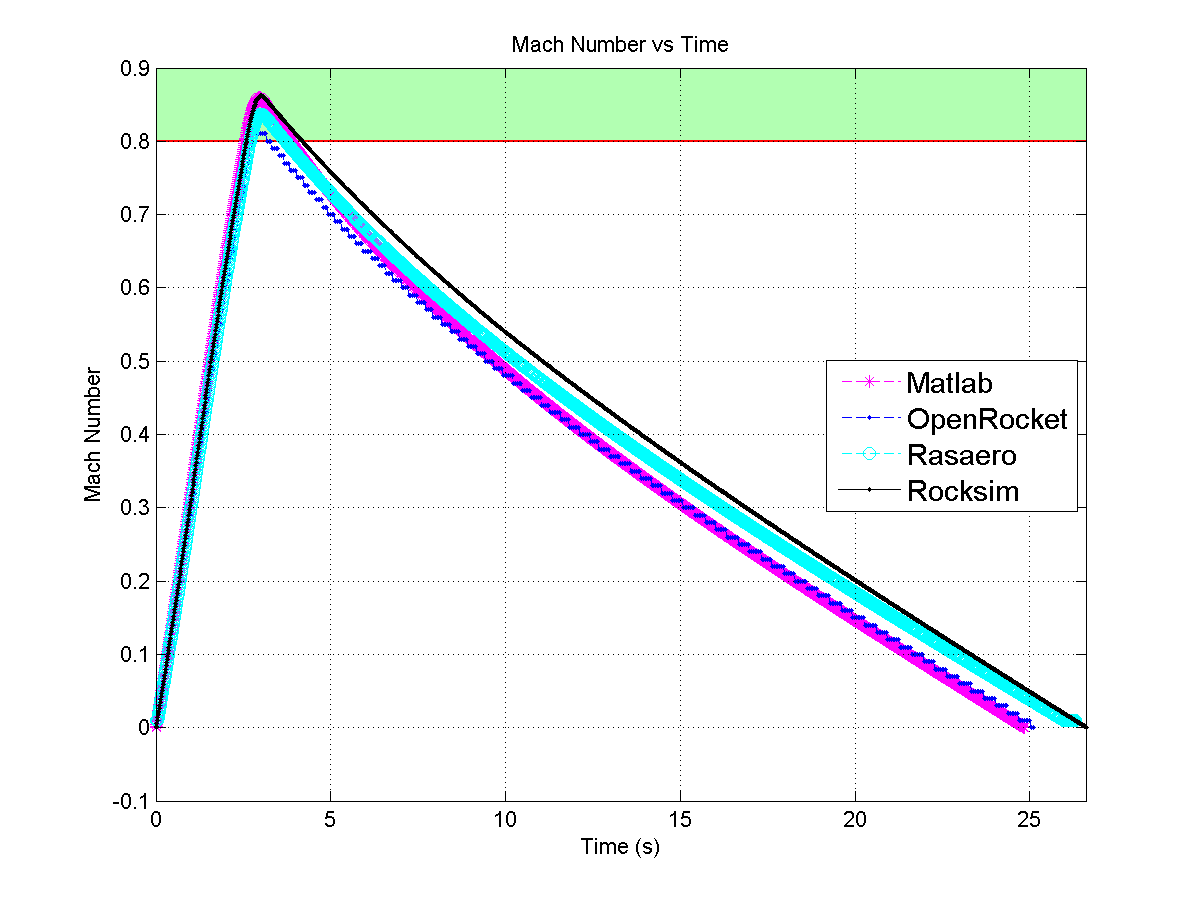
\includegraphics{images/plots/error_mach_plot.png}
\caption{Mass, Weight, and Thrust as a Function of Time
\label{error_mach_plot_label}}
\end{figure}

\begin{figure}[htbp]
\centering
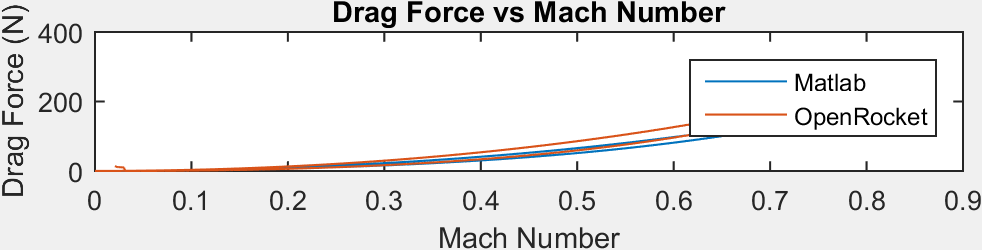
\includegraphics{images/plots/error_drag_plot.png}
\caption{Mass, Weight, and Thrust as a Function of Time
\label{error_drag_plot_label}}
\end{figure}

\subsubsection{Additional Plots}\label{additional-plots}

\begin{figure}[htbp]
\centering
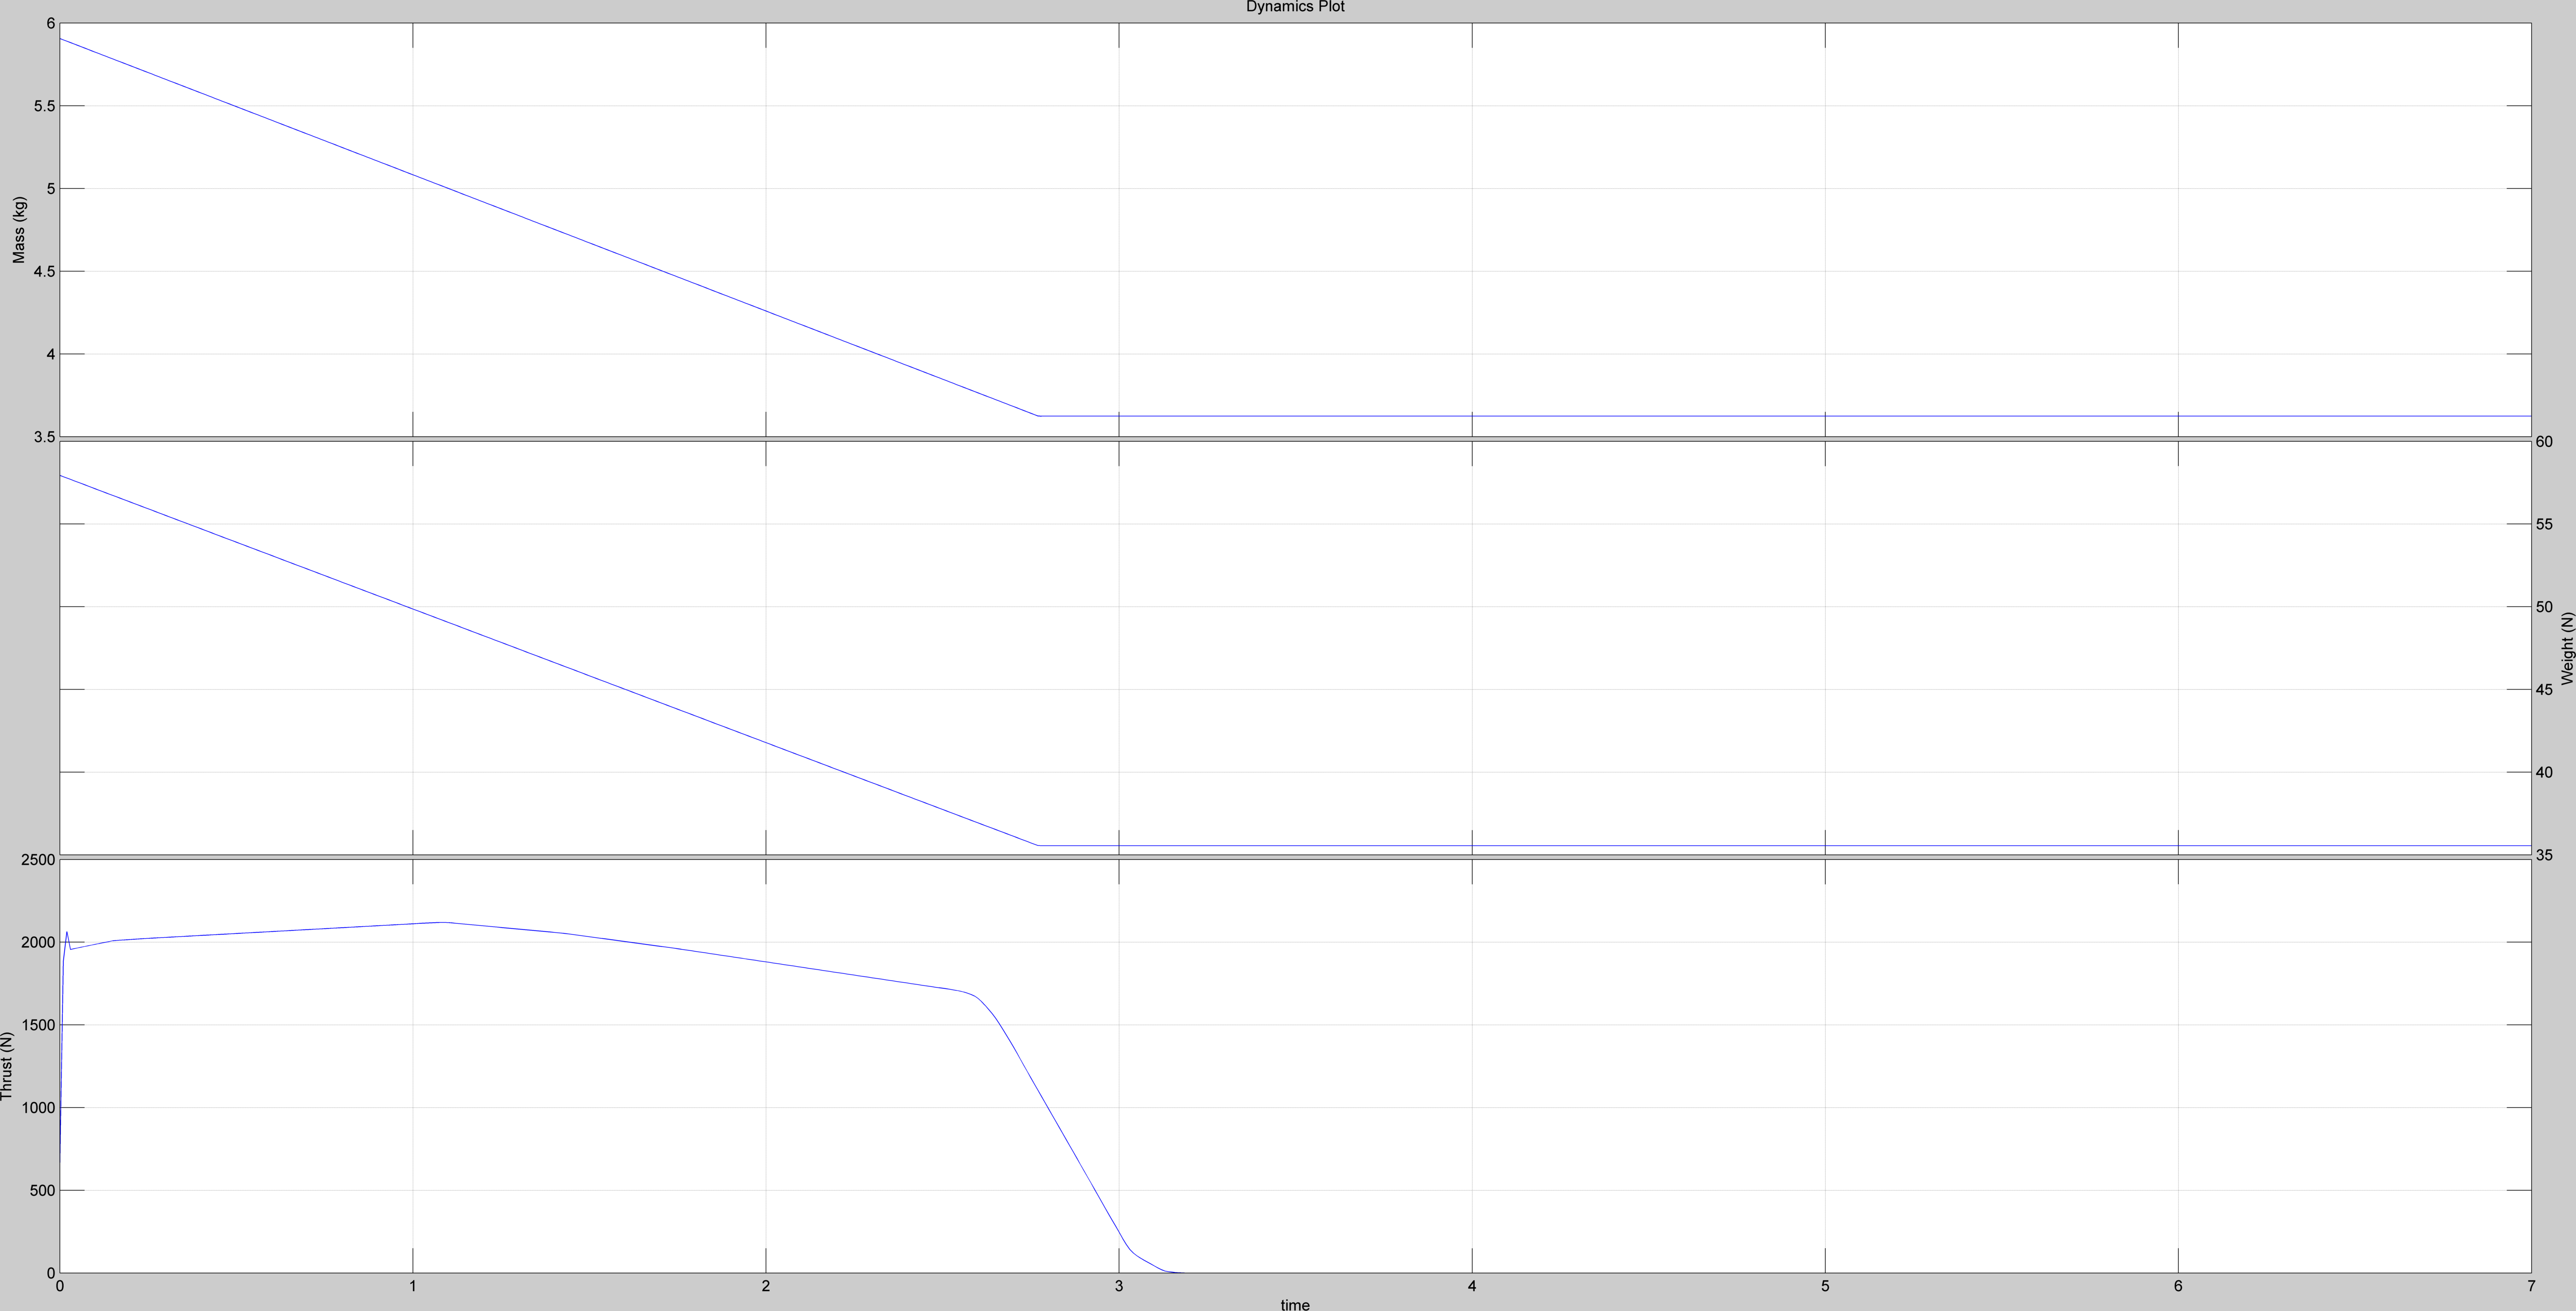
\includegraphics{images/plots/dynamics_plot.png}
\caption{Mass, Weight, and Thrust as a Function of Time
\label{dynamics_plot_label}}
\end{figure}

\begin{figure}[htbp]
\centering
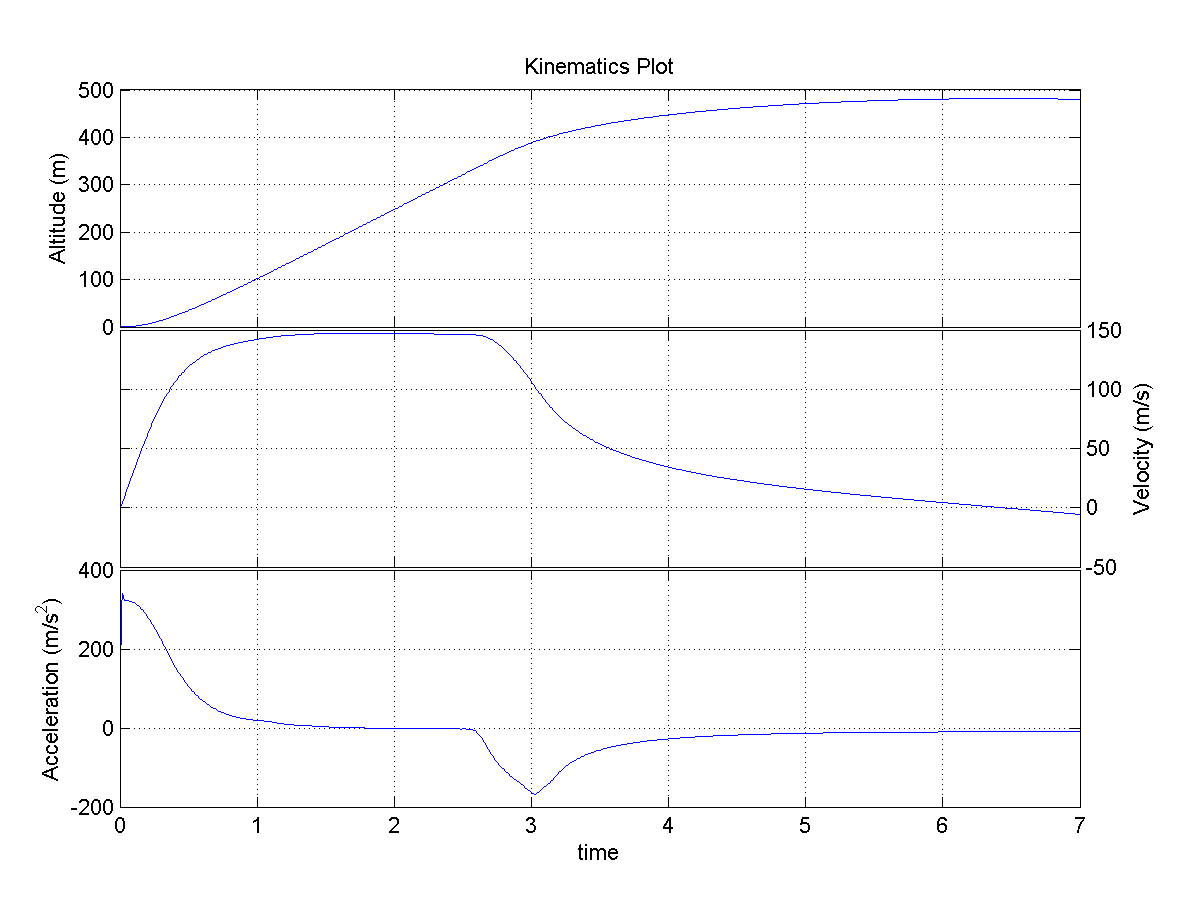
\includegraphics{images/plots/kinematics_plot.png}
\caption{Altitude, Velocity, and Acceleration as a Function of Time
\label{kinematics_plot_label}}
\end{figure}

\begin{figure}[htbp]
\centering
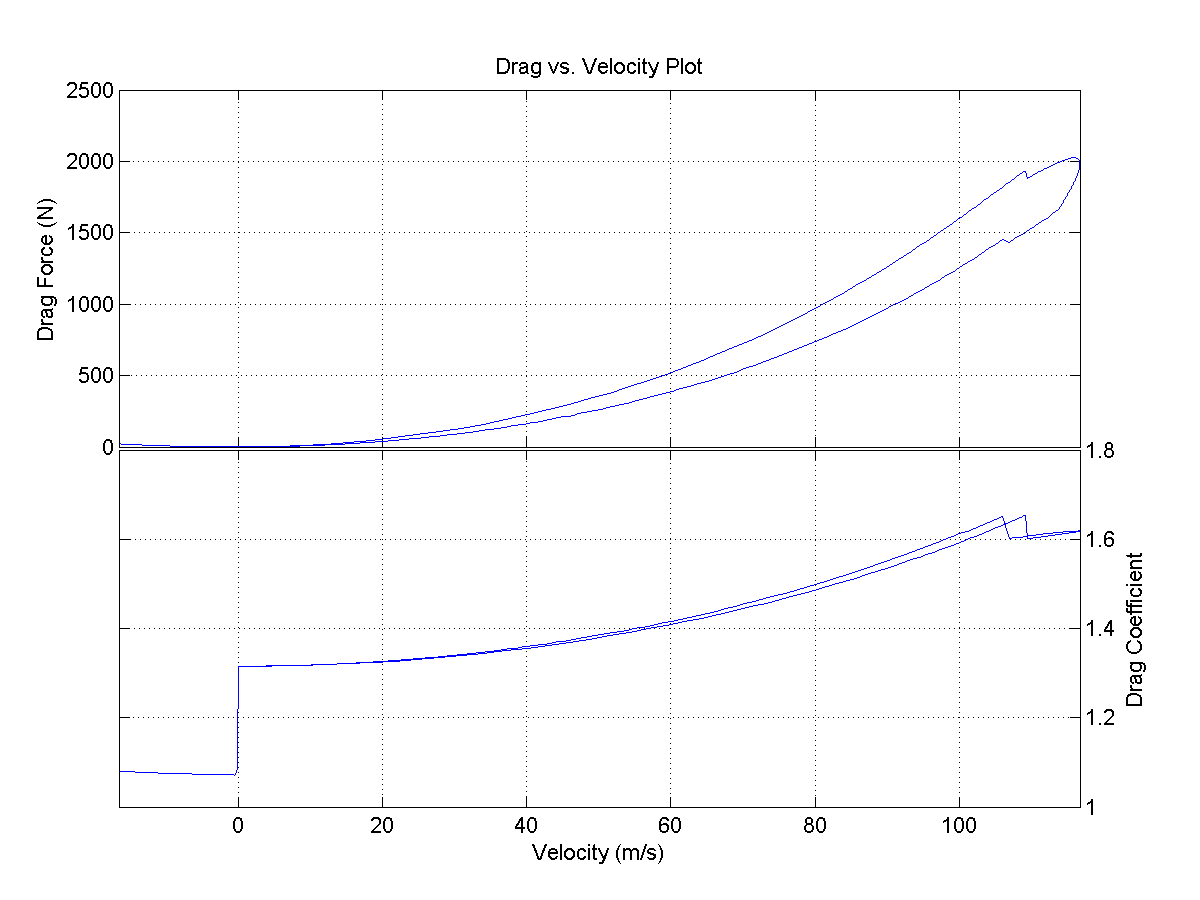
\includegraphics{images/plots/drag_v_velocity_plot.png}
\caption{Drag Force, Drag Coefficient, and Reynolds Number as a Function
of Velocity \label{drag_v_velocity_plot_label}}
\end{figure}

\begin{figure}[htbp]
\centering
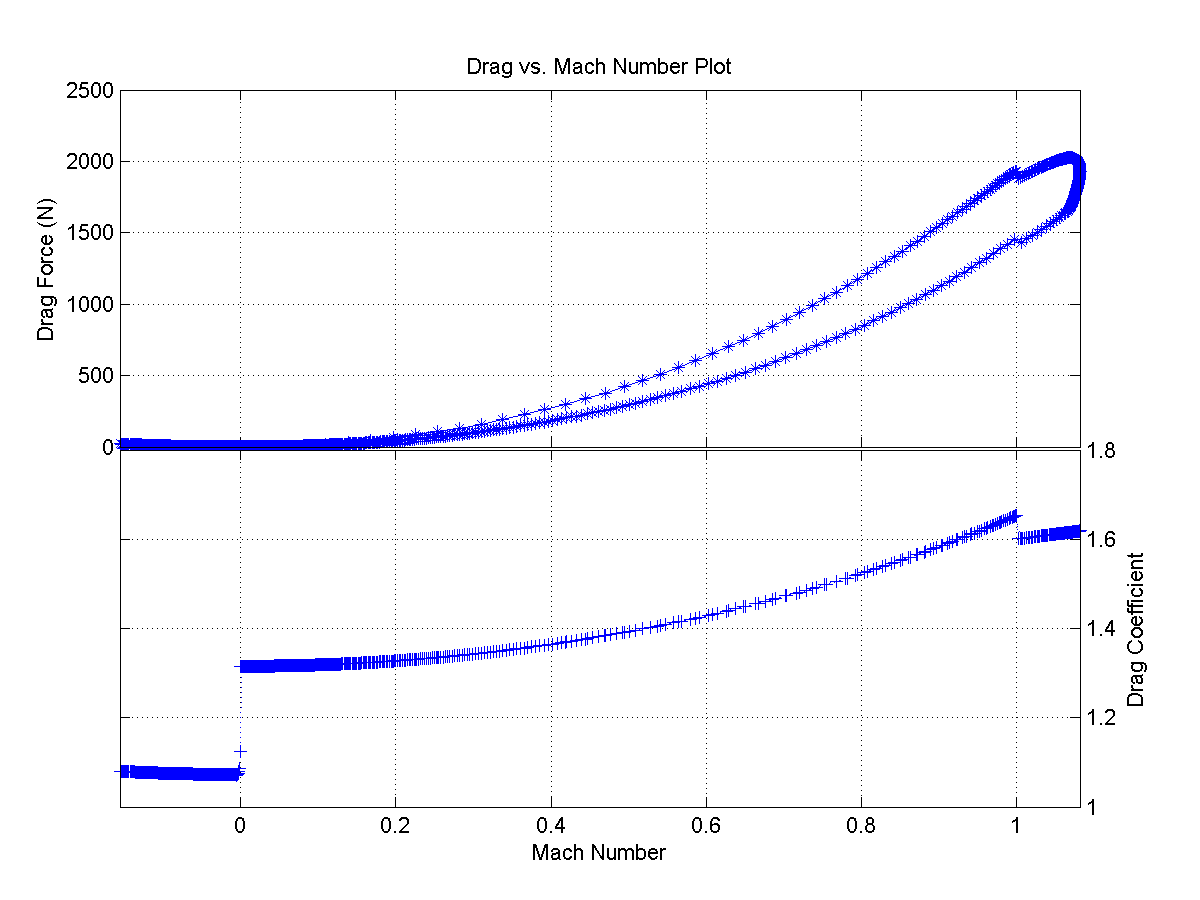
\includegraphics{images/plots/drag_v_mach.png}
\caption{Drag Force, Drag Coefficient, and Reynolds Number as a Function
of Mach Number \label{drag_v_mach_plot_label}}
\end{figure}

\begin{figure}[htbp]
\centering
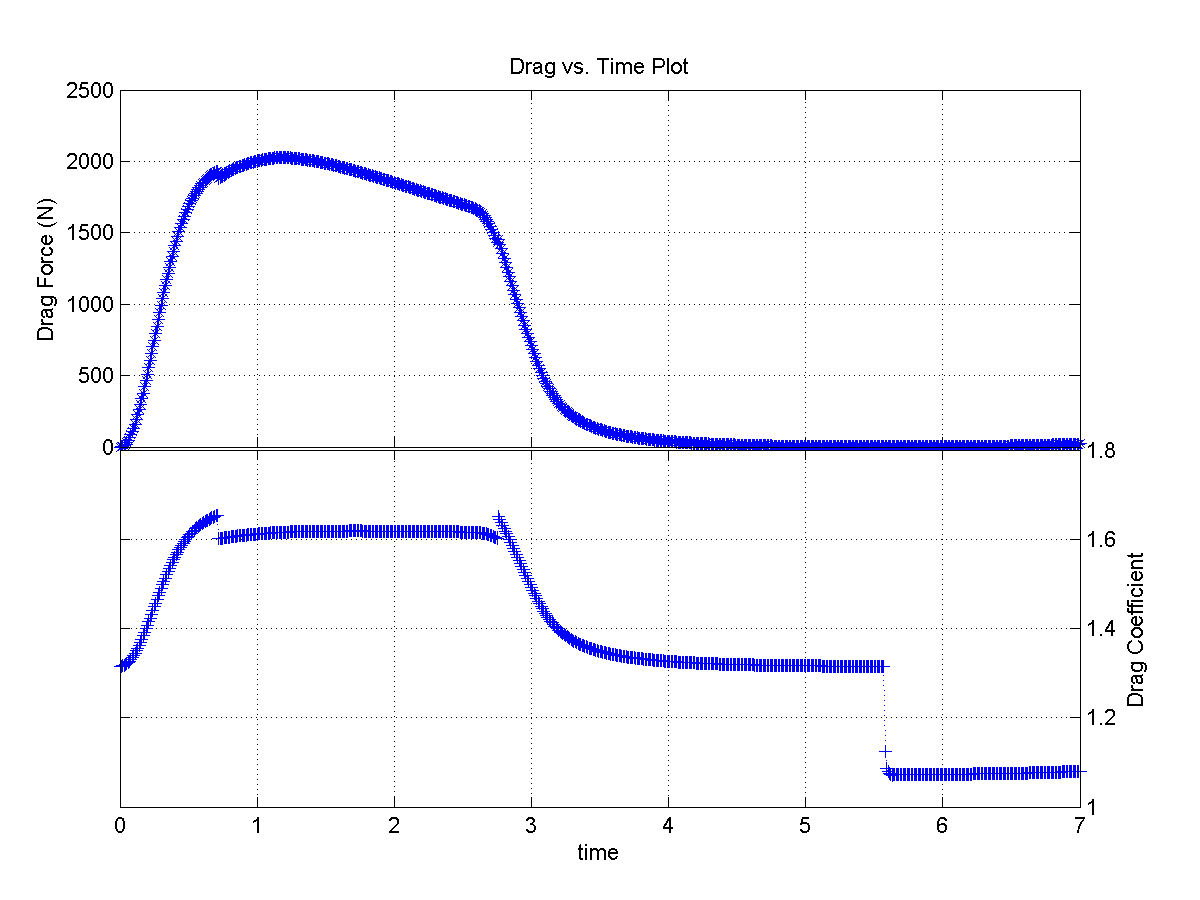
\includegraphics{images/plots/drag_plot.png}
\caption{Altitude, Velocity, and Acceleration as a Function of Time
\label{drag_plot_label}}
\end{figure}

\begin{figure}[htbp]
\centering
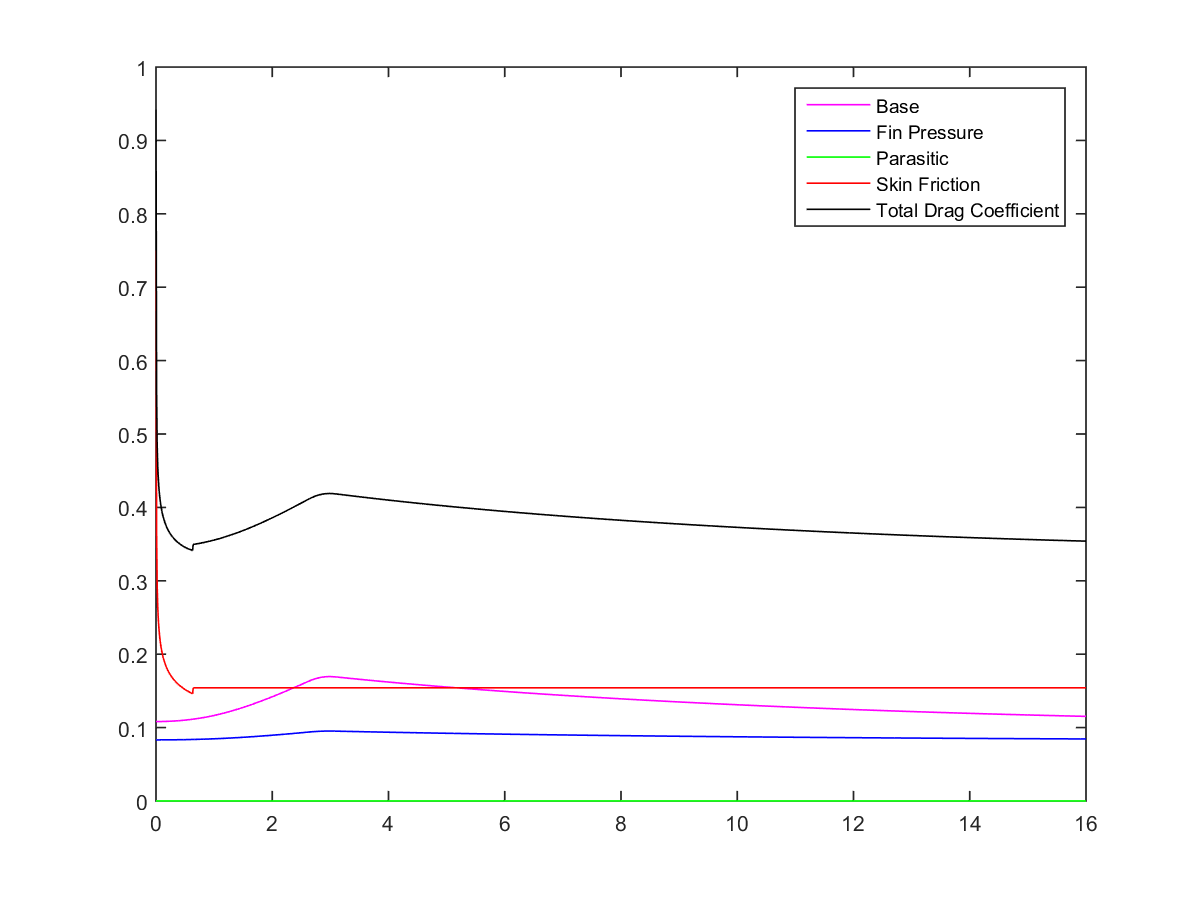
\includegraphics{images/plots/drag_coefficients.png}
\caption{Specific Drag Coefficients as a Function of Time
\label{drag_coefs_plot_label}}
\end{figure}

\begin{figure}[htbp]
\centering
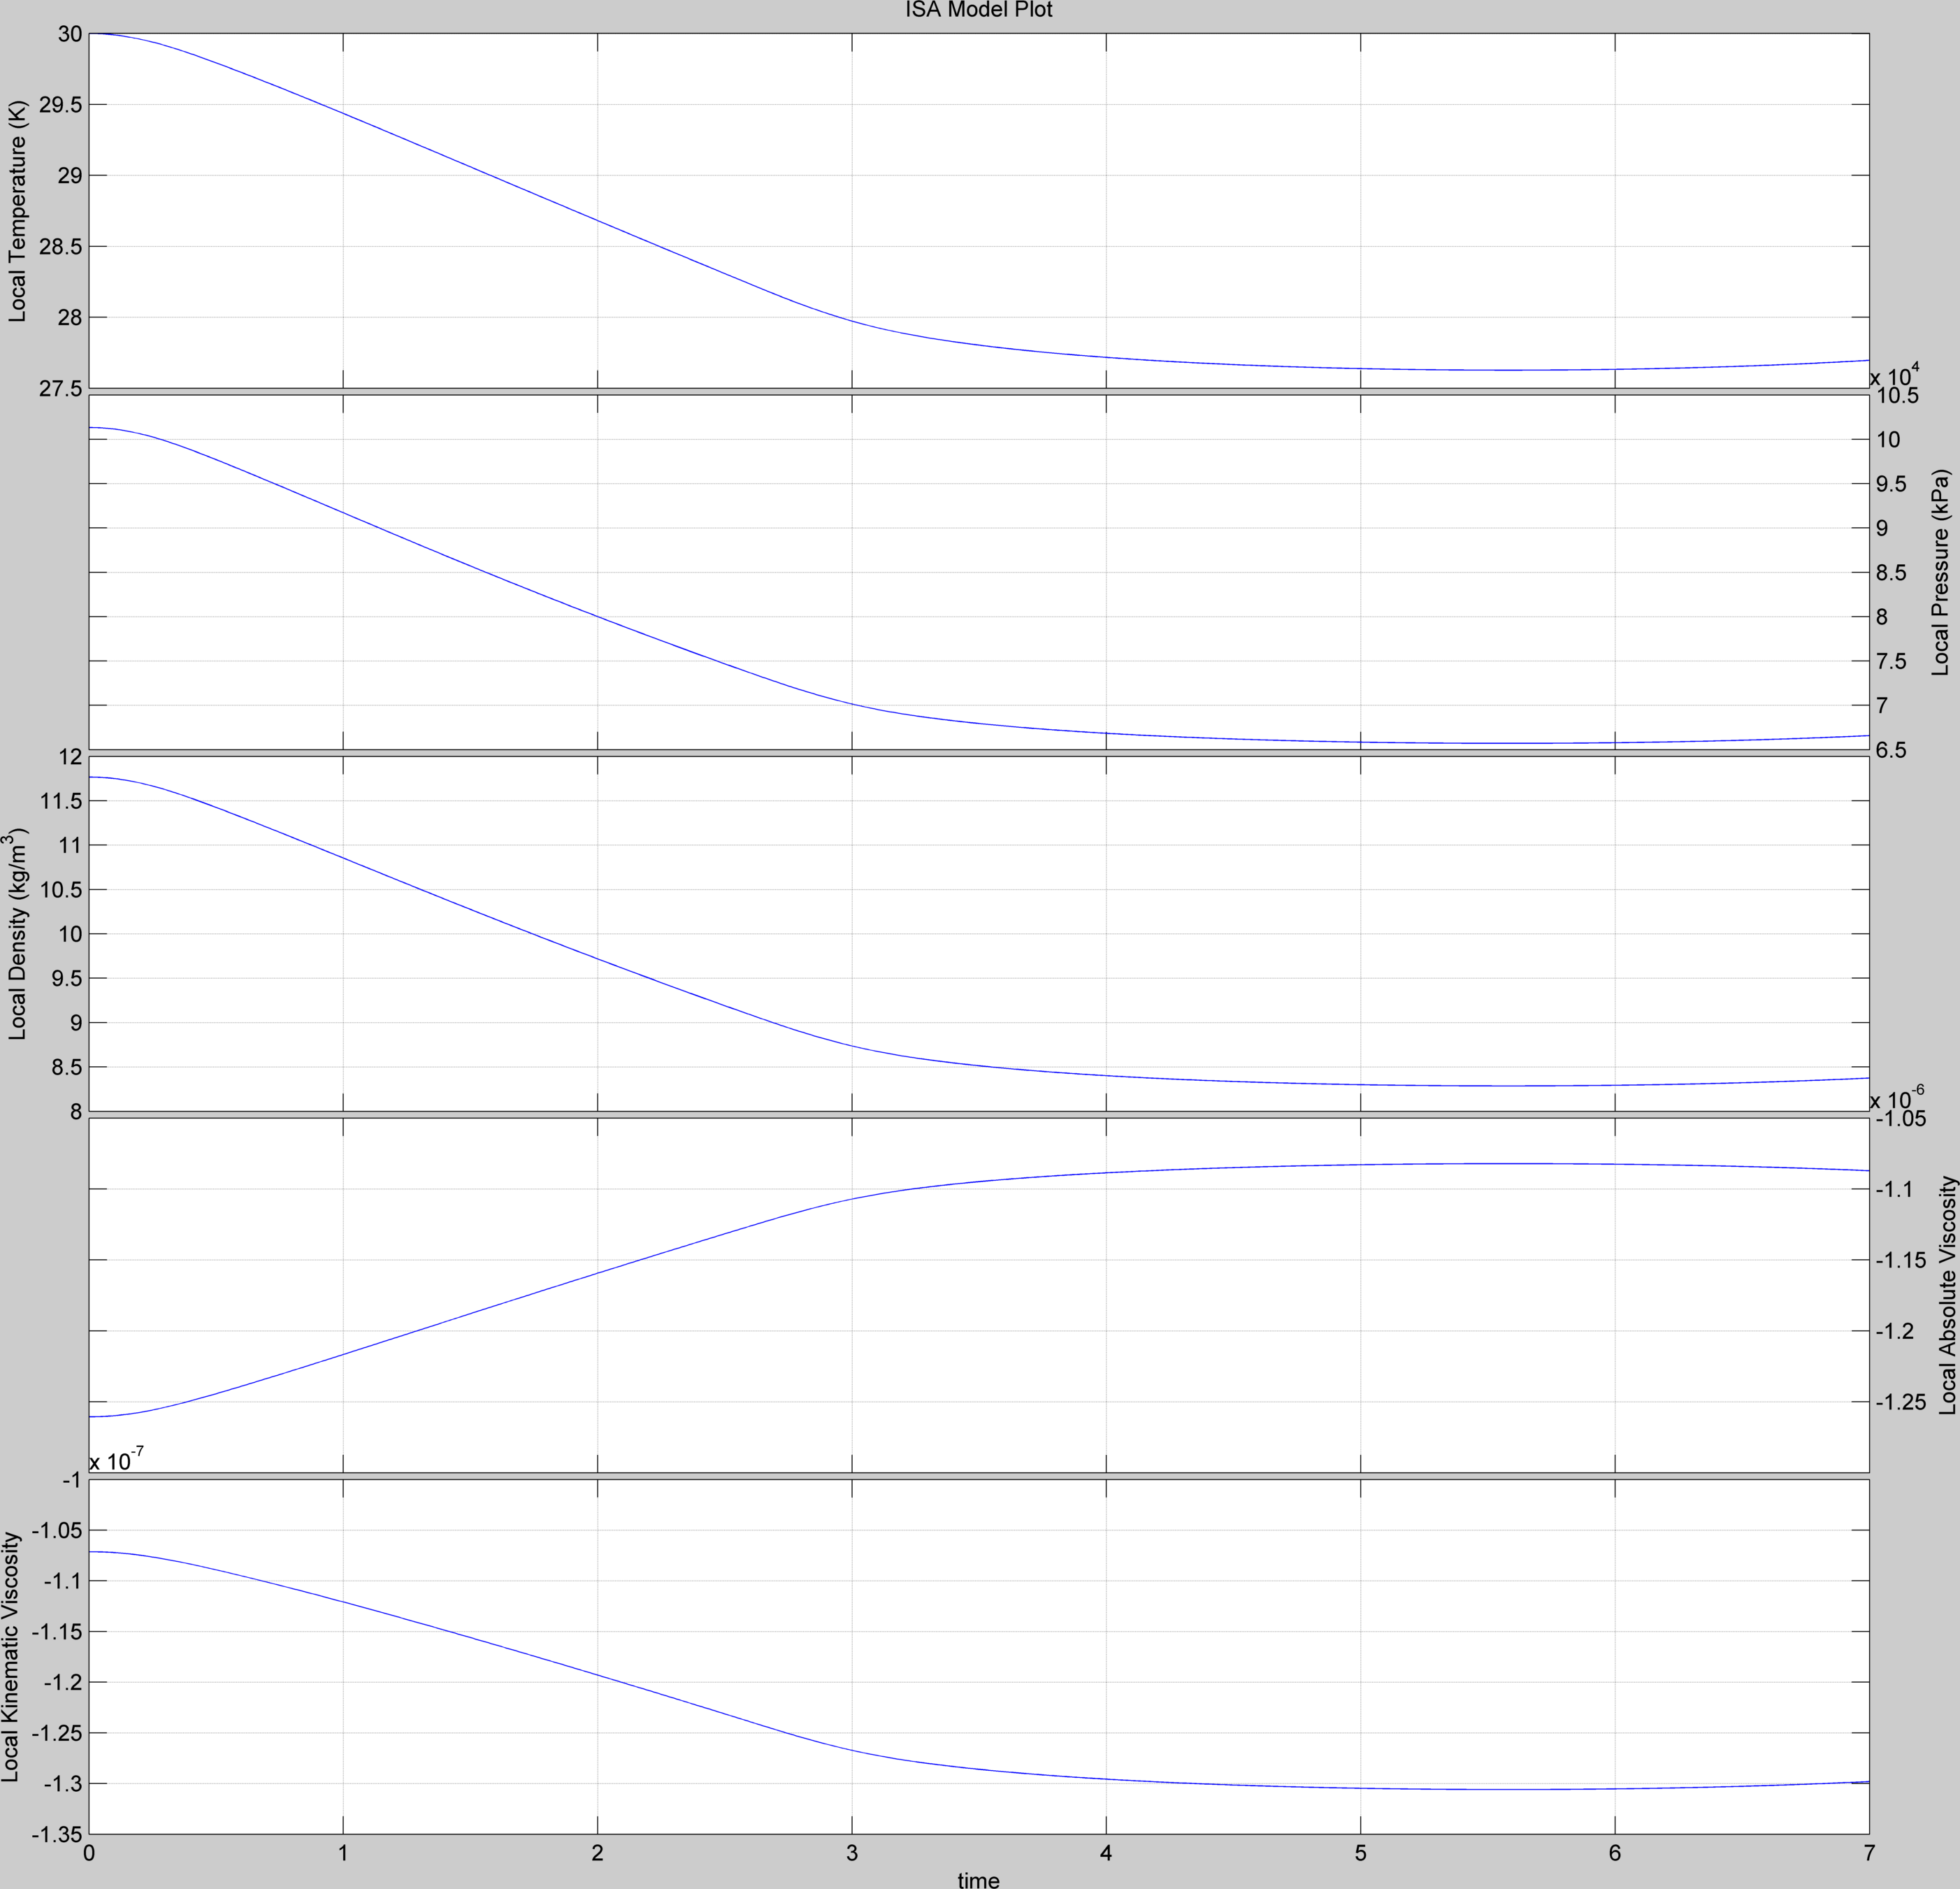
\includegraphics{images/plots/atmosphere_plot.png}
\caption{Altitude, Velocity, and Acceleration as a Function of Time
\label{atmosphere_plot_label}}
\end{figure}

\clearpage

\subsection{Raw Data}\label{raw-data}

See Appendix

\section{Conventions}\label{conventions}

\subsection{Data Model}\label{data-model}

\subsubsection{Data Store}\label{data-store}

\href{http://www.mathworks.com/help/simulink/data-stores.html}{Data
Stores}

\href{http://www.mathworks.com/help/simulink/slref/datastorememory.html}{Data
Store}

\href{http://www.mathworks.com/help/simulink/ug/when-to-use-a-data-store.html}{When
to Use a Data Store}

\href{http://www.mathworks.com/help/simulink/ug/data-store-examples.html}{Data
Store Examples}

\href{http://www.mathworks.com/help/simulink/ug/data-stores-and-software-verification.html}{Data
Stores and Software Verification} \textgreater{} see RTCA DO-331,
\href{http://www.rtca.org/Files/ListofAvailableDocsMarch2013.pdf}{``Model-Based
Development and Verification Supplement to DO-178C and DO-278A,''
Section MB.6.3.3.b.}

The \emph{Data Model} provides static and dynamics parameters as needed
by other models in the simulation.

\subsubsection{Static Parameters}\label{static-parameters-1}

Many parameters are constant throughout the simulation, notably the
structural dimensions. All structural dimensions are generated in the
CATIA Design and output to a spreadsheet, which the simulation will load
and place in a Matlab \emph{Map Container} instance.

\begin{quote}
http://www.mathworks.com/help/matlab/map-containers.html
\end{quote}

This instance can be accessed by multiple models to clearly and
effectively provide parameter access.

\paragraph{Spreadsheet Import and
Mapping}\label{spreadsheet-import-and-mapping}

\hyperdef{}{mycode}{\label{mycode}}
\begin{Shaded}
\begin{Highlighting}[numbers=left,,]
\NormalTok{function parametric_data_object = data_parametric_model()}
\CommentTok
\CommentTok
\CommentTok
\CommentTok{% Design Parameters for the Rocket are stored in a spreadsheet. }
\CommentTok{% These parameters will be accessed and passed along into the simulation to }
\CommentTok{% determine other parameters and ultimately to evaluate the performance of }
\CommentTok
\CommentTok{%--------------------------------------------------------------------------------}
\CommentTok{% References}
\CommentTok{% http://www.mathworks.com/help/simulink/ug/how-to-import-data-from-an-excel-spreadsheet.html}
\CommentTok{% http://www.mathworks.com/help/matlab/matlab_external/example-reading-excel-spreadsheet-data.html}
\CommentTok{%--------------------------------------------------------------------------------}

\CommentTok{% Import the data from Excel}
\NormalTok{[pnum,ptxt,praw] = xlsread(}\StringTok{'Parametric_Data.xlsm'}\NormalTok{,}\StringTok{'Matlab_Data'}\NormalTok{);}

\CommentTok{% Extract parameters from the imported data }
\NormalTok{keyset = ptxt(}\FloatTok{2}\NormalTok{:end,}\FloatTok{1}\NormalTok{);}
\NormalTok{valset = praw(}\FloatTok{2}\NormalTok{:end,}\FloatTok{2}\NormalTok{);}

\CommentTok{% initialize map object to store parametric data}
\NormalTok{parametric_data_object = containers.Map(keyset,valset);}

\NormalTok{end}
\end{Highlighting}
\end{Shaded}

\begin{verbatim}
\end{verbatim}

\subsubsection{Dynamic Parameters}\label{dynamic-parameters-1}

As discussed in the \emph{Dynamic Parameters} section, many parameters
are changing due to flight conditions. An additional \emph{Map
Container} instance is created to handle and deliver these changes to
the models that need them.

\subsection{Matlab Conventions}\label{matlab-conventions}

\subsection{Matlab/Simulink Libraries}\label{matlabsimulink-libraries}

\subsection{Overview}\label{overview-3}

The goal is to create a robust Simulink model that references Matlab
code from files that can be tracked by versioning software (Git). The
Matlab source should be editable and effect changes in the Simulink
model.

By a combination of both, full versioning control can be achieved in the
project.

\subsection{Creating a Library}\label{creating-a-library}

\begin{enumerate}
\def\labelenumi{\arabic{enumi}.}
\tightlist
\item
  Open Matlab
\item
  Open Simulink
\item
  Click File --\textgreater{} New --\textgreater{} Library
\end{enumerate}

\subsection{Add to path}\label{add-to-path}

Permanently add your workspace to the Matlab path. At the command
prompt:

\begin{verbatim}
>> pathtool
\end{verbatim}

\href{http://www3.nd.edu/~nancy/Math20550/Homework/matlabpath.pdf}{Alternatively,
try this howto}

\subsection{Add to Library Browser}\label{add-to-library-browser}

\href{http://www.mathworks.com/help/simulink/ug/adding-libraries-to-the-library-browser.html}{Add
to Library Browser}

\subsection{Simulink GOTCHAs}\label{simulink-gotchas}

\begin{itemize}
\tightlist
\item
  Atomic Units must be carefully employed to allow the simulation to run
\end{itemize}

\subsection{Importing Data}\label{importing-data}

Tabulated input data is relied upon to drive the simulation (see
\emph{Dynamic Parameters}). The following configuration is investigated
to support this smoothly

\href{http://www.mathworks.com/help/matlab/import_export/recommended-methods-for-importing-data.html}{Recommended
Methods for Importing Data}

\href{http://www.mathworks.com/help/simulink/import-data.html}{Load
Signal Data for Simulation}

\href{http://www.mathworks.com/help/simulink/ug/importing-signal-data-in-simulink.html}{Importing
Signal Data in Simulink}

\href{http://www.mathworks.com/help/simulink/ug/importing-data-structures-to-a-root-level-input-port.html}{Import
Data Structures}

\subsubsection{From File}\label{from-file}

The \emph{From File} block in Simulink allows incremental loading of
data

\begin{quote}
The From File block reads data from a MAT-file and outputs the data as a
signal. The data is a sequence of samples. Each sample consists of a
time stamp and an associated data value.
\end{quote}

\href{http://www.mathworks.com/help/simulink/slref/fromfile.html}{From
File}

\subparagraph{Mat-File Versions}\label{mat-file-versions}

Data is read incrementally from Mat-File versions 7.3 and above
\href{http://www.mathworks.com/help/matlab/import_export/mat-file-versions.html}{Mat-file
Versions}

\paragraph{nD Lookup Tables}\label{nd-lookup-tables}

\paragraph{Specifying Time Data}\label{specifying-time-data}

\href{http://www.mathworks.com/help/simulink/ug/importing-data-structures-to-a-root-level-input-port.html\#bsuwoyk}{Specifying
Time Data in Simulink}

\subsection{Versioning for Matlab
Files}\label{versioning-for-matlab-files}

\subsubsection{Background}\label{background}

\begin{itemize}
\tightlist
\item
  Older versions allowed providing external `.m' file for the
  \emph{Matlab Function} block in Simulink
\item
  Newer versions are shifting towards the embedded model, where Matlab
  code is complied for execution on test hardware
\end{itemize}

\href{http://www.goddardconsulting.ca/simulink-using-embedded-matlab.html}{Naming
conventions in Simulink for Matlab files changed after 2011A}

\paragraph{Interpreted Matlab
Function}\label{interpreted-matlab-function}

\emph{Interpreted Matlab Function} blocks are used to reference Matlab
files so they can be versioned in Git. \emph{Interpreted Matlab
Function} blocks only accept one input and one output, therefore we must
pass an array as input and an array as output. The contents of the array
will contain our variables of interest. \emph{(De))Mux} and \emph{Bus}
blocks may be useful to streamline the model.

\begin{enumerate}
\def\labelenumi{\arabic{enumi}.}
\tightlist
\item
  Write your Matlab function
\item
  Create a Simulink Model
\item
  Add the \emph{Interpreted Matlab Function} block
\item
  Double-click the added block, and enter the name of your function as
  directed. Select `OK'
\item
  Right-click the block, expand the `Mask', and select `Create Mask'
\item
  Add the following in the `Icon Drawing Commands' box
  \textsubscript{\textsubscript{\textsubscript{ disp(`function\_name')
  }}}
\item
  Add a \emph{Mux} block to combine your inports into a single input
  array, and a \emph{Demux} port to unpack your output array into
  outports
\end{enumerate}

\subsubsection{Versioning for Libraries}\label{versioning-for-libraries}

\begin{itemize}
\tightlist
\item
  Saving files as libraries and following the existing use cases in the
  documentation will allow robust versioning and collaboration workflow
\end{itemize}

\subsubsection{Unit Testing}\label{unit-testing-1}

\paragraph{Simulink Unit Testing}\label{simulink-unit-testing}

\subparagraph{Model Referencing}\label{model-referencing}

Model Referencing shall be used to test all libraries for expected
behavior.

\begin{enumerate}
\def\labelenumi{\arabic{enumi}.}
\tightlist
\item
  Create a Test Model in which you drag the Library
\item
  Provide all test inputs and output assertion
\item
  Create another model to contain all the test cases created in \emph{2}
\item
  From the \emph{Simulink Library}, drag a \emph{Model Reference} block
\item
  Edit the \emph{Model Reference} block, providing the name of the Test
  Model created in \emph{2}
\item
  Run the model created in \emph{3} to verify the model referencing was
  successful
\end{enumerate}

More information:

\begin{itemize}
\tightlist
\item
  http://www.mathworks.com/videos/getting-started-with-model-referencing-68918.html
\item
  http://www.mathworks.com/help/simulink/ug/creating-a-model-reference.html
\item
  http://www.mathworks.com/help/simulink/slref/model.html
\end{itemize}

\subsection{Exporting Images}\label{exporting-images}

High quality figures brings a great deal of value to a report. Simulink
Models and Matlab figures can be exported to scalable vector graphics
and PDF formats at high quality.

\subsubsection{GhostScript}\label{ghostscript}

\href{http://www.ghostscript.com/}{GhostScript} is needed to handle the
EPS format. It can be downloaded
\href{http://www.ghostscript.com/download/}{here}.

\subsubsection{GhostScript and GIMP}\label{ghostscript-and-gimp}

GIMP has problems opening EPS files with the default configuration.
Follow the instructions
\href{http://blog.tjitjing.com/index.php/2013/05/solution-error-open-eps-in-gimp-64-bit-with-ghostscript.html}{here}
to fix GhostScript in GIMP

\subsubsection{Exporting Figures}\label{exporting-figures}

\href{http://www.mathworks.com/matlabcentral/fileexchange/23629-export-fig}{export-fig}
is a Matlab library which provides functions to output figures to
various formats

\subsubsection{Exporting Simulink
Models}\label{exporting-simulink-models}

\href{https://truongnghiem.wordpress.com/2010/07/07/export-simulink-models-to-publication-quality-figures/}{export
Simulink models to publication-quality figures}

\href{https://truongnghiem.wordpress.com/2010/05/28/more-on-publication-quality-graphics-in-matlab/}{publication
quality graphics in Matlab}

\href{http://www.mathworks.com/matlabcentral/fileexchange/4638-laprint}{LaPrint}

\href{http://www.mathworks.com/matlabcentral/answers/94951-how-do-i-save-my-simulink-model-as-a-tiff-or-jpeg-image}{Howto}

\subsection{File Organization}\label{file-organization}

\begin{itemize}
\tightlist
\item
  data
\item
  documentation
\item
  functions
\item
  libraries
\item
  models
\item
  referencing
\item
  scripts
\item
  testing
\end{itemize}

\subsubsection{data}\label{data}

\paragraph{\texorpdfstring{data \(\rightarrow\)
csv}{data \textbackslash{}rightarrow csv}}\label{data-rightarrow-csv}

\subsubsection{documentation}\label{documentation}

\begin{itemize}
\tightlist
\item
  documentation

  \begin{itemize}
  \tightlist
  \item
    images
  \item
    template
  \end{itemize}
\end{itemize}

The \emph{documentation} folder contains all markdown files with project
documentation. It also contains

\paragraph{\texorpdfstring{documentation \(\rightarrow\)
images}{documentation \textbackslash{}rightarrow images}}\label{documentation-rightarrow-images}

Contains all images used in the documentation

\paragraph{\texorpdfstring{documentation \(\rightarrow\)
template}{documentation \textbackslash{}rightarrow template}}\label{documentation-rightarrow-template}

Contains LaTeX/Pandoc/Markdown template and styling files

\paragraph{functions}\label{functions}

\paragraph{libraries}\label{libraries}

\paragraph{models}\label{models}

\paragraph{referencing}\label{referencing}

\paragraph{scripts}\label{scripts}

\paragraph{testing}\label{testing}

\subsection{Naming Conventions}\label{naming-conventions}

\subsubsection{Variables}\label{variables}

All variables must be lowercase, separated by underscores

e.g.

\begin{verbatim}
wet_motor_weight
\end{verbatim}

\subsubsection{Functions}\label{functions-1}

All \emph{Matlab Functions} must be CamelCase

e.g.

\begin{verbatim}
DynamicWeightCalculation
\end{verbatim}

\subsubsection{Models}\label{models-1}

All \emph{Matlab Model} names must be CamelCase, and end in the word
`Model'

e.g.

\begin{verbatim}
DynamicWeightCalculationModel
\end{verbatim}

\subsubsection{Libraries}\label{libraries-1}

All \emph{Matlab Library} names must be CamelCase, and end in the word
`Library'

e.g.

\begin{verbatim}
DynamicWeightCalculationLibrary
\end{verbatim}

\section{Documentation Conventions}\label{documentation-conventions}

\subsection{Markdown}\label{markdown}

Markdown is a markup language that is meant to be easy to read and easy
to write, as well as easy to convert to HTML, LaTeX, PDF, and other
output types.

\subsection{Python}\label{python}

Python is used to enable additional filters which handle features
currently not supported out-of-the-box by Pandoc

\href{https://www.python.org/downloads/windows/}{Download Python for
Windows here}

\subsection{Pandoc}\label{pandoc}

Pandoc is a document converter that in our case is useful in converting
the Markdown (.md) files into PDF and HTML

\href{http://pandoc.org/README.html}{The User Guide is very helpful}

\subsection{Haskell}\label{haskell}

Haskell is useful in this environment to do some custom scripting

\subsection{LaTeX}\label{latex}

LaTeX is a powerful typesetting language useful for academic writing.
Its mathematical expressions are particularly useful for this report.

\subsection{Citations}\label{citations}

\href{http://www.chriskrycho.com/2015/academic-markdown-and-citations.html}{Excellent
citation discussion}

\href{http://blog.wuzzeb.org/posts/2012-06-15-bibtex-and-pandoc.html}{Haskell
and Bibtex in Pandoc}

\href{https://gist.github.com/marcelofernandez/3264858}{IEEE CSL File}
\href{https://gist.github.com/dnguyen85/d41b0f0bba387c1c31b7}{Another
IEEE CSL File}

\subsection{Equations}\label{equations}

Wrap functions as follows to enable automatic numbering:

\begin{verbatim}
\begin{equation}
\label{my_equation}
f(x) = \int \cdot e^{xy}
\end{equation}
\end{verbatim}

You can refer to the equation by the label you assigned to it

\begin{verbatim}
This comment refers to equation \ref{my_equation}
\end{verbatim}

\href{http://stackoverflow.com/questions/25042901/how-to-use-latex-equation-environment-in-pandoc-markdown}{LaTeX
equations in Markdown+Pandoc}

\subsection{Figures}\label{figures}

To automatically number figures, use the following syntax to insert an
image:

\begin{verbatim}
[rocket_drag_model_overview]: images/rocket_drag_model_overview.png "Rocket Drag Model Overview" 
![Rocket Drag Model Overview \label{rocket_drag_model_overview_label}][rocket_drag_model_overview] 
\end{verbatim}

Then, in your pandoc command, add the lof variable:

\begin{verbatim}
pandoc -s ... -V lof=lof
\end{verbatim}

You can refer to the figure by the label you assigned to it

\begin{verbatim}
This comment refers to Figure \ref{rocket_drag_model_overview_label}
\end{verbatim}

\subsection{Tables}\label{tables}

To automatically number tables and add captions, add the \emph{capt-of}
package to your preamble

\begin{verbatim}
\usepackage{capt-of}
\end{verbatim}

Then, in your pandoc command, add the lot variable:

\begin{verbatim}
pandoc -s ... -V lot=lot
\end{verbatim}

\section*{References}\label{references}
\addcontentsline{toc}{section}{References}

\hyperdef{}{refs}{\label{refs}}
\hyperdef{}{ref-box2009}{\label{ref-box2009}}
{[}1{]} Simon Box Christopher M. Bishop and H. Hunt, ``Estimating the
dynamic and aerodynamic paramters of passively controlled high power
rockets for flight simulaton,'' February 2009.

\hyperdef{}{ref-niskanen2013}{\label{ref-niskanen2013}}
{[}2{]} S. Niskanen, ``OpenRocket technical documentation (development
of an open source model rocket simulation software),'' PhD thesis.

\hyperdef{}{ref-cavcarISA}{\label{ref-cavcarISA}}
{[}3{]} V. as a Function of Temperature, ``Mustafa cavcar.'' Online,
September-2006.

\hyperdef{}{ref-barrowman}{\label{ref-barrowman}}
{[}4{]} J. Barrowman, ``Calculating the center of pressure of a model
rocket,'' 1998.

\hyperdef{}{ref-munson2013}{\label{ref-munson2013}}
{[}5{]} H. Munson Okiishi, \emph{Munson fundamentals of fluid
mechanics}. Cambridge, Mass: John Wiley; Sons Inc, 2013.

\hyperdef{}{ref-mandell1973}{\label{ref-mandell1973}}
{[}6{]} G. J. C. Mandell Gordon K. and W. P. Bengen., \emph{Topics in
advanced model rocketry}. Cambridge, Mass: MIT Press, 1973.

\hyperdef{}{ref-gregorek}{\label{ref-gregorek}}
{[}7{]} D. G. M. Gregorek, ``Aerodynamic drag of model rockets,''
\emph{ESTES INDUSTRIES INC.}, 1970.

\hyperdef{}{ref-galejs}{\label{ref-galejs}}
{[}8{]} R. Galejs, ``What barrowman left out,'' 1999.

\end{document}
